\chapter{Desarrollo de la interfaz de usuario}
En Ingeniería del Software nos enseñaron que para añadir una interfaz de usuario a un sistema ya hecho no había que modificar el sistema ya existente. Hay metodologías que empiezan haciendo una interfaz de usuario ``vacía'' y, a partir de ahí, van añadiéndole funcionalidad a sus botones. En nuestro caso hemos optado por el primer principio, ya que nos pareció la forma más natural de hacerlo. A continuación, explicaré cómo hice para conectar la aplicación web que he desarrollado como interfaz de usuario con el programa \texttt{Python} que calcula el horario.

\section{Herramienta usada}
Actualmente, hay un montón de tecnologías o herramientas para hacer todo tipo de interfaces de usuario. Me limité a buscar herramientas para \texttt{Python}, pues así podía integrar de forma muy sencilla todo el trabajo previo ya realizado en este lenguaje. Si hubiese usado otras herramientas, tendría que haber un puente para intercambiar información entre ambas, lo que podría suponer un cuello de botella. Por ejemplo, para conectar Python con un servidor NodeJS, se tienen que hacer JSON que reciben como parámetro y devuelven ambas partes para intercambiar información. Hay herramientas en el mercado que están así implementadas, como por ejemplo, la Restful API de Wazuh (\url{https://github.com/wazuh/wazuh-api}). 

A la hora de hacer una interfaz de usuario en \textit{Python} tenía dos opciones: o bien hacer una interfaz usando \texttt{PyQt} (\url{https://wiki.python.org/moin/PyQt}) o bien hacer una \textit{aplicación web}. Finalmente, me decanté por hacer una aplicación web por las varias razones. En primer lugar, una aplicación web \textit{responsive} puede usarse tanto desde un teléfono móvil como desde un ordenador. Además, el uso de una aplicación web permite que varias personas trabajen a la vez sobre la misma usando una base de datos centralizada, en lugar de tener una copia de los datos en cada ordenador. Otra ventaja de hacer una aplicación web es que el programador se puede abstraer del sistema operativo, ya que se ejecutará en un navegador. Así, en lugar de hacer una aplicación para cada sistema operativo, sólo se hace una que se dejará ejecutando en un servidor y a la que los usuarios accederán desde su PC. Lo único que debe preocupar al programador es el navegador que se use, sobre todo si algún usuario aún sigue usando \textit{Internet Explorer}.

Cuando ya decidí qué tipo de interfaz de usuario haría, pasé a pensar con qué \textbf{herramienta} iba a hacerla. Estuve pensando en \texttt{Flask} (\url{http://flask.pocoo.org/}), pero finalmente lo descarté porque es un \textit{framework} que se usa (o se debería de usar) para hacer aplicaciones sencillas. De hecho, su eslogan es \textit{A Python Microframework}. A parte de esto, su documentación es un poco pobre. También estuve pensando en \texttt{Django} (\url{https://www.djangoproject.com/}). \texttt{Django} es fácilmente escalable, con sólo cambiar una línea en un fichero de configuración y hacer algún que otro pequeño ajuste más podemos pasar de usar \texttt{SQLite3} a usar \texttt{PostgreeSQL}, es decir, podemos pasar de usar un gestor de base de datos de ``juguete'' a uno muy potente. Además, tiene una documentación buenísima que incluye un montón de ejemplos ya hechos, además de un montón de explicaciones con muchísimo detalle. Y no solo eso, tiene además una comunidad enorme detrás, por lo que cualquier problema que surja estará resuelto en internet con bastante probabilidad.

\begin{figure}
\centering
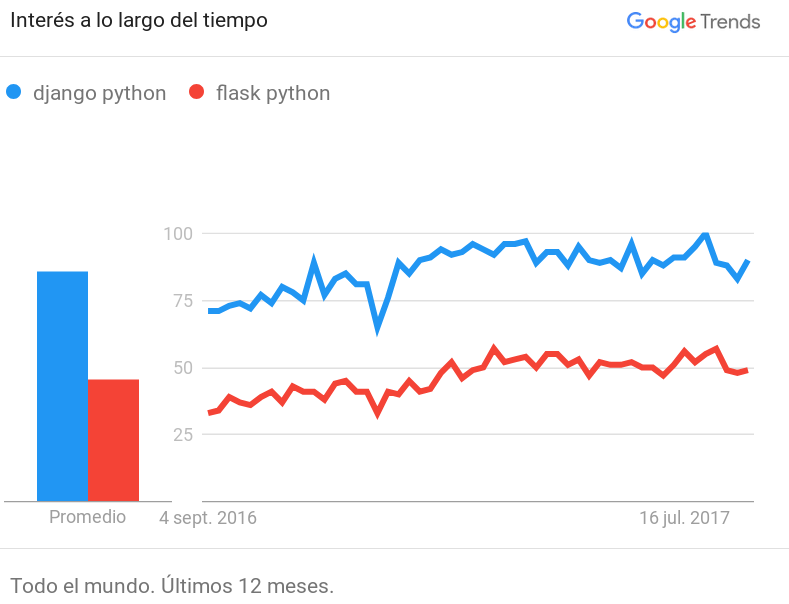
\includegraphics[width=0.7\textwidth]{img/django_flask_trends}
\caption{Interés sobre \texttt{Django} (en azul) y sobre \texttt{Flask} a lo largo del último año en todo el mundo. Datos: Google Trends (\url{https://g.co/trends/CgxUq})}
\label{djangoflasktrends}
\end{figure}

De hecho, si consultamos los datos ofrecidos por \textit{Google Trends} (\hyperref[djangoflasktrends]{Figura \ref*{djangoflasktrends}}) podemos ver que \texttt{Django} es mucho más popular que \texttt{Flask}. Esta es una razón más para elegir uno sobre el otro. ¿Por qué? Porque si un \textit{framework} es popular, significa que tendrá una comunidad que lo mantendrá y dará soporte durante mucho más tiempo. 

\subsection{Django}
\subsubsection{Instalación}
Para instalar \texttt{Django}, lo único que tenemos que hacer es ejecutar el siguiente comando:

\begin{minted}{shell-session}
$ sudo pip install django
\end{minted}

O, si sólo queremos instalar \texttt{Django} de forma local al proyecto y no en nuestro sistema, podemos crear un \texttt{\textit{virtualenv}} (\url{https://virtualenv.pypa.io/en/stable/}). Con esto, evitamos tener nuestro sistema lleno de paquetes que sólo hemos usado para una cosa concreta. Además, también nos da más flexibilidad, pues nos permite tener instalada una versión concreta de un paquete y evita colisiones entre paquetes. 

Al igual que \texttt{Django}, \texttt{virtualenv} se instala desde \texttt{pip}:

\begin{minted}{shell-session}
$ sudo pip install virtualenv
[sudo] password for marta: 
Collecting virtualenv
  Downloading virtualenv-15.1.0-py2.py3-none-any.whl (1.8MB)
    100% |================================| 1.8MB 374kB/s 
Installing collected packages: virtualenv
Successfully installed virtualenv-15.1.0
\end{minted}

Una vez instalado, para crear un \texttt{virtualenv} en la carpeta de nuestro proyecto ejecutamos el siguiente comando:

\begin{minted}{shell-session}
$ virtualenv ENV
Using base prefix '/usr'
New python executable in ENV/bin/python
Installing setuptools, pip, wheel...done.
\end{minted}

Donde \texttt{ENV} es la carpeta en la que queremos crear el \texttt{virtualenv}. 

Una vez creado, veremos los siguientes directorios:

% \begin{minted}{shell-session}
% $ ls -l
% total 16
% drwxr-xr-x 2 marta marta 4096 sep  5 19:57 bin
% drwxr-xr-x 2 marta marta 4096 sep  5 19:57 include
% drwxr-xr-x 3 marta marta 4096 sep  5 19:57 lib
% -rw-r--r-- 1 marta marta   60 sep  5 19:57 pip-selfcheck.json
% \end{minted}

\begin{enumerate}[---]
\item Los directorios \texttt{lib} e \texttt{include} contienen librerías que instalamos en el \texttt{virtualenv}. Recién creado, sólo contienen el intérprete de \texttt{python}.
\item El directorio \texttt{bin} guarda los ejecutables tantp de los paquetes que instalaremos en el \texttt{virtualenv} como los ejecutables que necesita \texttt{virutalenv} para funcionar.
\end{enumerate}

Un \texttt{virtualenv} recién creado necesita ser activado. Para ello, ejecutamos:

\begin{minted}{shell-session}
$ source bin/activate
\end{minted}

Nada más ejecutarlo, se modificará el shell para indicarnos que estamos dentro del \texttt{virtualenv}. Si queremos ``salir'' del mismo, basta con ejecutar:

\begin{minted}{shell-session}
$ deactivate
\end{minted}

Y volveremos a nuestra shell normal.

Volviendo a la instalación de \texttt{Django}, ahora que tenemos nuestro \texttt{virtualenv} listo podemos instalar \texttt{Django} sin usar sudo:

\begin{minted}{shell-session}
$ pip install Django
Collecting Django
  Downloading Django-1.11.5-py2.py3-none-any.whl (6.9MB)
    100% |=================================| 7.0MB 152kB/s 
Collecting pytz (from Django)
  Downloading pytz-2017.2-py2.py3-none-any.whl (484kB)
    100% |=================================| 491kB 788kB/s 
Installing collected packages: pytz, Django
Successfully installed Django-1.11.5 pytz-2017.2
\end{minted}

Para comprobar que \texttt{Django} se ha instalado correctamente, usamos el siguiente comando:

\begin{minted}{shell-session}
$ python -m django --version
1.11.5
\end{minted}

\subsubsection{Creando un proyecto}
Una de las cosas que más me gusta de \texttt{Django}, es que él solo automatiza un montón de tareas. Así, como ellos mismos dicen en su documentación, el programador puede centrarse en programar única y exclusivamente. Con otros \textit{framework} tendría que estar todo un día preparando un entorno de desarrollo antes de poder ponerme manos a la obra, en cambio, lo único que tengo que hacer es ejecutar el siguiente comando:

\begin{minted}{shell-session}
$ django-admin startproject NOMBRE
\end{minted}

donde \texttt{NOMBRE} es el nombre que queremos darle a nuestro proyecto.

Este comando nos crea toda la estructura de directorios necesaria para empezar a trabajar. Dicha estructura es la que se ve en la \hyperref[djangoprojectfolders]{Figura \ref*{djangoprojectfolders}}.

\begin{figure}
\centering
\scalebox{.7}{% Graphic for TeX using PGF
% Title: /home/marta/Diagrama1.dia
% Creator: Dia v0.97.3
% CreationDate: Thu Sep  7 22:53:00 2017
% For: marta
% \usepackage{tikz}
% The following commands are not supported in PSTricks at present
% We define them conditionally, so when they are implemented,
% this pgf file will use them.
\ifx\du\undefined
  \newlength{\du}
\fi
\setlength{\du}{15\unitlength}
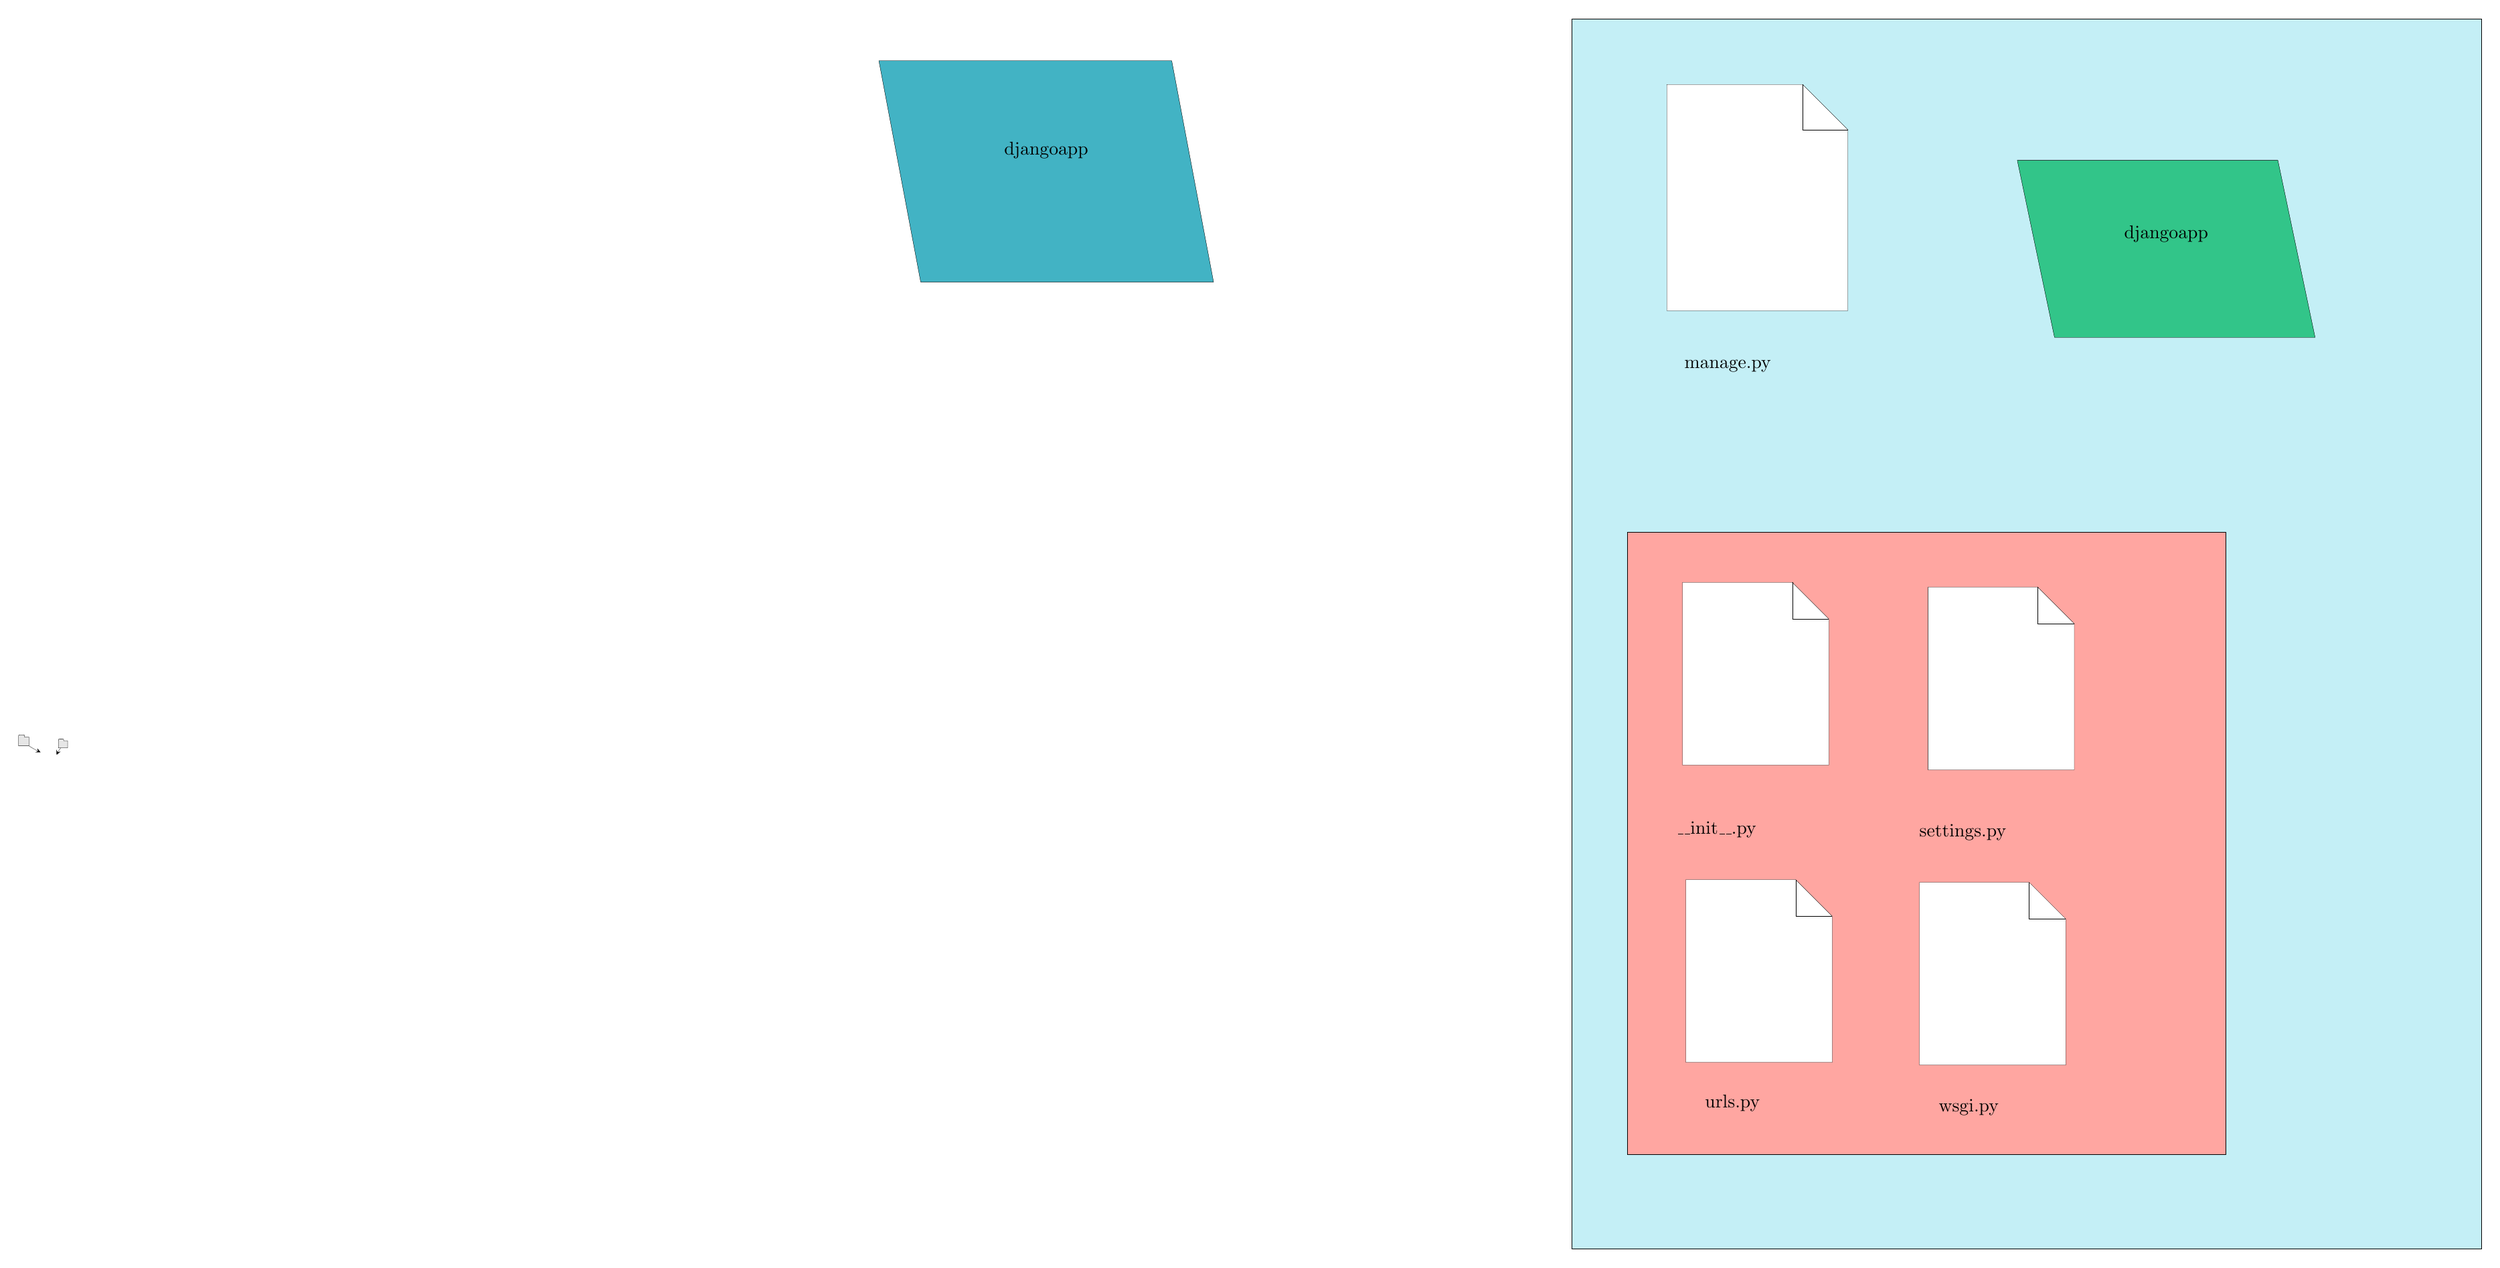
\begin{tikzpicture}
\pgftransformxscale{1.000000}
\pgftransformyscale{-1.000000}
\definecolor{dialinecolor}{rgb}{0.000000, 0.000000, 0.000000}
\pgfsetstrokecolor{dialinecolor}
\definecolor{dialinecolor}{rgb}{1.000000, 1.000000, 1.000000}
\pgfsetfillcolor{dialinecolor}
\pgfsetlinewidth{0.100000\du}
\pgfsetdash{}{0pt}
\pgfsetdash{}{0pt}
\pgfsetbuttcap
\pgfsetmiterjoin
\pgfsetlinewidth{0.100000\du}
\pgfsetbuttcap
\pgfsetmiterjoin
\pgfsetdash{}{0pt}
\definecolor{dialinecolor}{rgb}{0.901961, 0.901961, 0.901961}
\pgfsetfillcolor{dialinecolor}
\pgfpathmoveto{\pgfpoint{17.739413\du}{-13.924815\du}}
\pgfpathcurveto{\pgfpoint{17.739413\du}{-15.124814\du}}{\pgfpoint{17.739413\du}{-15.124814\du}}{\pgfpoint{18.533163\du}{-15.124814\du}}
\pgfpathcurveto{\pgfpoint{19.326913\du}{-15.124814\du}}{\pgfpoint{19.326913\du}{-15.124814\du}}{\pgfpoint{20.120663\du}{-15.124814\du}}
\pgfpathcurveto{\pgfpoint{20.914413\du}{-15.124814\du}}{\pgfpoint{20.914413\du}{-15.124814\du}}{\pgfpoint{20.914413\du}{-13.924815\du}}
\pgfpathcurveto{\pgfpoint{20.914413\du}{-13.924815\du}}{\pgfpoint{23.295663\du}{-13.924815\du}}{\pgfpoint{23.295663\du}{-13.924815\du}}
\pgfpathcurveto{\pgfpoint{23.295663\du}{-13.924815\du}}{\pgfpoint{23.295663\du}{-9.124814\du}}{\pgfpoint{23.295663\du}{-9.124814\du}}
\pgfpathcurveto{\pgfpoint{23.295663\du}{-9.124814\du}}{\pgfpoint{17.739413\du}{-9.124814\du}}{\pgfpoint{17.739413\du}{-9.124814\du}}
\pgfpathcurveto{\pgfpoint{17.739413\du}{-9.124814\du}}{\pgfpoint{17.739413\du}{-12.724814\du}}{\pgfpoint{17.739413\du}{-13.924815\du}}
\pgfusepath{fill}
\definecolor{dialinecolor}{rgb}{0.000000, 0.000000, 0.000000}
\pgfsetstrokecolor{dialinecolor}
\pgfpathmoveto{\pgfpoint{17.739413\du}{-13.924815\du}}
\pgfpathcurveto{\pgfpoint{17.739413\du}{-15.124814\du}}{\pgfpoint{17.739413\du}{-15.124814\du}}{\pgfpoint{18.533163\du}{-15.124814\du}}
\pgfpathcurveto{\pgfpoint{19.326913\du}{-15.124814\du}}{\pgfpoint{19.326913\du}{-15.124814\du}}{\pgfpoint{20.120663\du}{-15.124814\du}}
\pgfpathcurveto{\pgfpoint{20.914413\du}{-15.124814\du}}{\pgfpoint{20.914413\du}{-15.124814\du}}{\pgfpoint{20.914413\du}{-13.924815\du}}
\pgfpathcurveto{\pgfpoint{20.914413\du}{-13.924815\du}}{\pgfpoint{23.295663\du}{-13.924815\du}}{\pgfpoint{23.295663\du}{-13.924815\du}}
\pgfpathcurveto{\pgfpoint{23.295663\du}{-13.924815\du}}{\pgfpoint{23.295663\du}{-9.124814\du}}{\pgfpoint{23.295663\du}{-9.124814\du}}
\pgfpathcurveto{\pgfpoint{23.295663\du}{-9.124814\du}}{\pgfpoint{17.739413\du}{-9.124814\du}}{\pgfpoint{17.739413\du}{-9.124814\du}}
\pgfpathcurveto{\pgfpoint{17.739413\du}{-9.124814\du}}{\pgfpoint{17.739413\du}{-12.724814\du}}{\pgfpoint{17.739413\du}{-13.924815\du}}
\pgfusepath{stroke}
\pgfsetlinewidth{0.010000\du}
\pgfsetbuttcap
\pgfsetmiterjoin
\pgfsetdash{}{0pt}
\definecolor{dialinecolor}{rgb}{0.000000, 0.000000, 0.000000}
\pgfsetstrokecolor{dialinecolor}
\pgfpathmoveto{\pgfpoint{17.739413\du}{-13.924815\du}}
\pgfpathcurveto{\pgfpoint{17.739413\du}{-15.124814\du}}{\pgfpoint{17.739413\du}{-15.124814\du}}{\pgfpoint{18.533163\du}{-15.124814\du}}
\pgfpathcurveto{\pgfpoint{19.326913\du}{-15.124814\du}}{\pgfpoint{19.326913\du}{-15.124814\du}}{\pgfpoint{20.120663\du}{-15.124814\du}}
\pgfpathcurveto{\pgfpoint{20.914413\du}{-15.124814\du}}{\pgfpoint{20.914413\du}{-15.124814\du}}{\pgfpoint{20.914413\du}{-13.924815\du}}
\pgfpathcurveto{\pgfpoint{20.914413\du}{-13.924815\du}}{\pgfpoint{23.295663\du}{-13.924815\du}}{\pgfpoint{23.295663\du}{-13.924815\du}}
\pgfpathcurveto{\pgfpoint{23.295663\du}{-13.924815\du}}{\pgfpoint{23.295663\du}{-9.124814\du}}{\pgfpoint{23.295663\du}{-9.124814\du}}
\pgfpathcurveto{\pgfpoint{23.295663\du}{-9.124814\du}}{\pgfpoint{17.739413\du}{-9.124814\du}}{\pgfpoint{17.739413\du}{-9.124814\du}}
\pgfpathcurveto{\pgfpoint{17.739413\du}{-9.124814\du}}{\pgfpoint{17.739413\du}{-12.724814\du}}{\pgfpoint{17.739413\du}{-13.924815\du}}
\pgfusepath{stroke}
\pgfsetlinewidth{0.100000\du}
\pgfsetbuttcap
\pgfsetmiterjoin
\pgfsetdash{}{0pt}
\definecolor{dialinecolor}{rgb}{0.258824, 0.701961, 0.768627}
\pgfsetfillcolor{dialinecolor}
\fill (17.739413\du,-9.124814\du)--(16.945663\du,-13.324813\du)--(22.501913\du,-13.324813\du)--(23.295663\du,-9.124814\du)--cycle;
\definecolor{dialinecolor}{rgb}{0.000000, 0.000000, 0.000000}
\pgfsetstrokecolor{dialinecolor}
\draw (17.739413\du,-9.124814\du)--(16.945663\du,-13.324813\du)--(22.501913\du,-13.324813\du)--(23.295663\du,-9.124814\du)--cycle;
\pgfsetlinewidth{0.010000\du}
\pgfsetbuttcap
\pgfsetmiterjoin
\pgfsetdash{}{0pt}
\definecolor{dialinecolor}{rgb}{0.000000, 0.000000, 0.000000}
\pgfsetstrokecolor{dialinecolor}
\draw (17.739413\du,-9.124814\du)--(16.945663\du,-13.324813\du)--(22.501913\du,-13.324813\du)--(23.295663\du,-9.124814\du)--cycle;
% setfont left to latex
\definecolor{dialinecolor}{rgb}{1.000000, 1.000000, 1.000000}
\pgfsetstrokecolor{dialinecolor}
\node at (20.120663\du,-11.624814\du){djangoapp};
\pgfsetlinewidth{0.100000\du}
\pgfsetdash{}{0pt}
\pgfsetdash{}{0pt}
\pgfsetmiterjoin
\definecolor{dialinecolor}{rgb}{0.768627, 0.937255, 0.964706}
\pgfsetfillcolor{dialinecolor}
\fill (30.095663\du,-14.124814\du)--(30.095663\du,9.225186\du)--(47.345663\du,9.225186\du)--(47.345663\du,-14.124814\du)--cycle;
\definecolor{dialinecolor}{rgb}{0.000000, 0.000000, 0.000000}
\pgfsetstrokecolor{dialinecolor}
\draw (30.095663\du,-14.124814\du)--(30.095663\du,9.225186\du)--(47.345663\du,9.225186\du)--(47.345663\du,-14.124814\du)--cycle;
\pgfsetlinewidth{0.100000\du}
\pgfsetdash{}{0pt}
\pgfsetdash{}{0pt}
\pgfsetbuttcap
{
\definecolor{dialinecolor}{rgb}{0.000000, 0.000000, 0.000000}
\pgfsetfillcolor{dialinecolor}
% was here!!!
\pgfsetarrowsend{stealth}
\definecolor{dialinecolor}{rgb}{0.000000, 0.000000, 0.000000}
\pgfsetstrokecolor{dialinecolor}
\pgfpathmoveto{\pgfpoint{23.338714\du}{-9.126739\du}}
\pgfpatharc{123}{115}{51.064311\du and 51.064311\du}
\pgfusepath{stroke}
}
\pgfsetlinewidth{0.100000\du}
\pgfsetdash{}{0pt}
\pgfsetdash{}{0pt}
\pgfsetbuttcap
\pgfsetmiterjoin
\pgfsetlinewidth{0.100000\du}
\pgfsetbuttcap
\pgfsetmiterjoin
\pgfsetdash{}{0pt}
\definecolor{dialinecolor}{rgb}{1.000000, 1.000000, 1.000000}
\pgfsetfillcolor{dialinecolor}
\fill (31.895663\du,-12.874814\du)--(34.471913\du,-12.874814\du)--(35.330663\du,-12.016064\du)--(35.330663\du,-8.581064\du)--(31.895663\du,-8.581064\du)--cycle;
\definecolor{dialinecolor}{rgb}{0.000000, 0.000000, 0.000000}
\pgfsetstrokecolor{dialinecolor}
\draw (31.895663\du,-12.874814\du)--(34.471913\du,-12.874814\du)--(35.330663\du,-12.016064\du)--(35.330663\du,-8.581064\du)--(31.895663\du,-8.581064\du)--cycle;
\pgfsetbuttcap
\pgfsetmiterjoin
\pgfsetdash{}{0pt}
\definecolor{dialinecolor}{rgb}{0.000000, 0.000000, 0.000000}
\pgfsetstrokecolor{dialinecolor}
\draw (34.471913\du,-12.874814\du)--(34.471913\du,-12.016064\du)--(35.330663\du,-12.016064\du)--(35.330663\du,-12.016064\du);
% setfont left to latex
\definecolor{dialinecolor}{rgb}{0.000000, 0.000000, 0.000000}
\pgfsetstrokecolor{dialinecolor}
\node[anchor=west] at (32.113163\du,-7.527939\du){manage.py};
% setfont left to latex
\definecolor{dialinecolor}{rgb}{0.000000, 0.000000, 0.000000}
\pgfsetstrokecolor{dialinecolor}
\node[anchor=west] at (40.465663\du,-10.649814\du){};
% setfont left to latex
\definecolor{dialinecolor}{rgb}{0.000000, 0.000000, 0.000000}
\pgfsetstrokecolor{dialinecolor}
\node[anchor=west] at (33.613163\du,-10.727939\du){};
\pgfsetlinewidth{0.100000\du}
\pgfsetdash{}{0pt}
\pgfsetdash{}{0pt}
\pgfsetbuttcap
\pgfsetmiterjoin
\pgfsetlinewidth{0.100000\du}
\pgfsetbuttcap
\pgfsetmiterjoin
\pgfsetdash{}{0pt}
\definecolor{dialinecolor}{rgb}{0.901961, 0.901961, 0.901961}
\pgfsetfillcolor{dialinecolor}
\pgfpathmoveto{\pgfpoint{39.251913\du}{-11.914814\du}}
\pgfpathcurveto{\pgfpoint{39.251913\du}{-12.874814\du}}{\pgfpoint{39.251913\du}{-12.874814\du}}{\pgfpoint{39.958163\du}{-12.874814\du}}
\pgfpathcurveto{\pgfpoint{40.664413\du}{-12.874814\du}}{\pgfpoint{40.664413\du}{-12.874814\du}}{\pgfpoint{41.370663\du}{-12.874814\du}}
\pgfpathcurveto{\pgfpoint{42.076913\du}{-12.874814\du}}{\pgfpoint{42.076913\du}{-12.874814\du}}{\pgfpoint{42.076913\du}{-11.914814\du}}
\pgfpathcurveto{\pgfpoint{42.076913\du}{-11.914814\du}}{\pgfpoint{44.195663\du}{-11.914814\du}}{\pgfpoint{44.195663\du}{-11.914814\du}}
\pgfpathcurveto{\pgfpoint{44.195663\du}{-11.914814\du}}{\pgfpoint{44.195663\du}{-8.074814\du}}{\pgfpoint{44.195663\du}{-8.074814\du}}
\pgfpathcurveto{\pgfpoint{44.195663\du}{-8.074814\du}}{\pgfpoint{39.251913\du}{-8.074814\du}}{\pgfpoint{39.251913\du}{-8.074814\du}}
\pgfpathcurveto{\pgfpoint{39.251913\du}{-8.074814\du}}{\pgfpoint{39.251913\du}{-10.954814\du}}{\pgfpoint{39.251913\du}{-11.914814\du}}
\pgfusepath{fill}
\definecolor{dialinecolor}{rgb}{0.000000, 0.000000, 0.000000}
\pgfsetstrokecolor{dialinecolor}
\pgfpathmoveto{\pgfpoint{39.251913\du}{-11.914814\du}}
\pgfpathcurveto{\pgfpoint{39.251913\du}{-12.874814\du}}{\pgfpoint{39.251913\du}{-12.874814\du}}{\pgfpoint{39.958163\du}{-12.874814\du}}
\pgfpathcurveto{\pgfpoint{40.664413\du}{-12.874814\du}}{\pgfpoint{40.664413\du}{-12.874814\du}}{\pgfpoint{41.370663\du}{-12.874814\du}}
\pgfpathcurveto{\pgfpoint{42.076913\du}{-12.874814\du}}{\pgfpoint{42.076913\du}{-12.874814\du}}{\pgfpoint{42.076913\du}{-11.914814\du}}
\pgfpathcurveto{\pgfpoint{42.076913\du}{-11.914814\du}}{\pgfpoint{44.195663\du}{-11.914814\du}}{\pgfpoint{44.195663\du}{-11.914814\du}}
\pgfpathcurveto{\pgfpoint{44.195663\du}{-11.914814\du}}{\pgfpoint{44.195663\du}{-8.074814\du}}{\pgfpoint{44.195663\du}{-8.074814\du}}
\pgfpathcurveto{\pgfpoint{44.195663\du}{-8.074814\du}}{\pgfpoint{39.251913\du}{-8.074814\du}}{\pgfpoint{39.251913\du}{-8.074814\du}}
\pgfpathcurveto{\pgfpoint{39.251913\du}{-8.074814\du}}{\pgfpoint{39.251913\du}{-10.954814\du}}{\pgfpoint{39.251913\du}{-11.914814\du}}
\pgfusepath{stroke}
\pgfsetlinewidth{0.010000\du}
\pgfsetbuttcap
\pgfsetmiterjoin
\pgfsetdash{}{0pt}
\definecolor{dialinecolor}{rgb}{0.000000, 0.000000, 0.000000}
\pgfsetstrokecolor{dialinecolor}
\pgfpathmoveto{\pgfpoint{39.251913\du}{-11.914814\du}}
\pgfpathcurveto{\pgfpoint{39.251913\du}{-12.874814\du}}{\pgfpoint{39.251913\du}{-12.874814\du}}{\pgfpoint{39.958163\du}{-12.874814\du}}
\pgfpathcurveto{\pgfpoint{40.664413\du}{-12.874814\du}}{\pgfpoint{40.664413\du}{-12.874814\du}}{\pgfpoint{41.370663\du}{-12.874814\du}}
\pgfpathcurveto{\pgfpoint{42.076913\du}{-12.874814\du}}{\pgfpoint{42.076913\du}{-12.874814\du}}{\pgfpoint{42.076913\du}{-11.914814\du}}
\pgfpathcurveto{\pgfpoint{42.076913\du}{-11.914814\du}}{\pgfpoint{44.195663\du}{-11.914814\du}}{\pgfpoint{44.195663\du}{-11.914814\du}}
\pgfpathcurveto{\pgfpoint{44.195663\du}{-11.914814\du}}{\pgfpoint{44.195663\du}{-8.074814\du}}{\pgfpoint{44.195663\du}{-8.074814\du}}
\pgfpathcurveto{\pgfpoint{44.195663\du}{-8.074814\du}}{\pgfpoint{39.251913\du}{-8.074814\du}}{\pgfpoint{39.251913\du}{-8.074814\du}}
\pgfpathcurveto{\pgfpoint{39.251913\du}{-8.074814\du}}{\pgfpoint{39.251913\du}{-10.954814\du}}{\pgfpoint{39.251913\du}{-11.914814\du}}
\pgfusepath{stroke}
\pgfsetlinewidth{0.100000\du}
\pgfsetbuttcap
\pgfsetmiterjoin
\pgfsetdash{}{0pt}
\definecolor{dialinecolor}{rgb}{0.196078, 0.772549, 0.537255}
\pgfsetfillcolor{dialinecolor}
\fill (39.251913\du,-8.074814\du)--(38.545663\du,-11.434814\du)--(43.489413\du,-11.434814\du)--(44.195663\du,-8.074814\du)--cycle;
\definecolor{dialinecolor}{rgb}{0.000000, 0.000000, 0.000000}
\pgfsetstrokecolor{dialinecolor}
\draw (39.251913\du,-8.074814\du)--(38.545663\du,-11.434814\du)--(43.489413\du,-11.434814\du)--(44.195663\du,-8.074814\du)--cycle;
\pgfsetlinewidth{0.010000\du}
\pgfsetbuttcap
\pgfsetmiterjoin
\pgfsetdash{}{0pt}
\definecolor{dialinecolor}{rgb}{0.000000, 0.000000, 0.000000}
\pgfsetstrokecolor{dialinecolor}
\draw (39.251913\du,-8.074814\du)--(38.545663\du,-11.434814\du)--(43.489413\du,-11.434814\du)--(44.195663\du,-8.074814\du)--cycle;
% setfont left to latex
\definecolor{dialinecolor}{rgb}{1.000000, 1.000000, 1.000000}
\pgfsetstrokecolor{dialinecolor}
\node at (41.370663\du,-10.034814\du){djangoapp};
\pgfsetlinewidth{0.100000\du}
\pgfsetdash{}{0pt}
\pgfsetdash{}{0pt}
\pgfsetmiterjoin
\definecolor{dialinecolor}{rgb}{1.000000, 0.650980, 0.631373}
\pgfsetfillcolor{dialinecolor}
\fill (31.145663\du,-4.374814\du)--(31.145663\du,7.425186\du)--(42.499256\du,7.425186\du)--(42.499256\du,-4.374814\du)--cycle;
\definecolor{dialinecolor}{rgb}{0.000000, 0.000000, 0.000000}
\pgfsetstrokecolor{dialinecolor}
\draw (31.145663\du,-4.374814\du)--(31.145663\du,7.425186\du)--(42.499256\du,7.425186\du)--(42.499256\du,-4.374814\du)--cycle;
\pgfsetlinewidth{0.100000\du}
\pgfsetdash{}{0pt}
\pgfsetdash{}{0pt}
\pgfsetbuttcap
{
\definecolor{dialinecolor}{rgb}{0.000000, 0.000000, 0.000000}
\pgfsetfillcolor{dialinecolor}
% was here!!!
\pgfsetarrowsend{stealth}
\definecolor{dialinecolor}{rgb}{0.000000, 0.000000, 0.000000}
\pgfsetstrokecolor{dialinecolor}
\pgfpathmoveto{\pgfpoint{40.435680\du}{-8.025240\du}}
\pgfpatharc{217}{204}{19.089005\du and 19.089005\du}
\pgfusepath{stroke}
}
\pgfsetlinewidth{0.100000\du}
\pgfsetdash{}{0pt}
\pgfsetdash{}{0pt}
\pgfsetbuttcap
\pgfsetmiterjoin
\pgfsetlinewidth{0.100000\du}
\pgfsetbuttcap
\pgfsetmiterjoin
\pgfsetdash{}{0pt}
\definecolor{dialinecolor}{rgb}{1.000000, 1.000000, 1.000000}
\pgfsetfillcolor{dialinecolor}
\fill (32.195663\du,-3.424814\du)--(34.276913\du,-3.424814\du)--(34.970663\du,-2.731064\du)--(34.970663\du,0.043936\du)--(32.195663\du,0.043936\du)--cycle;
\definecolor{dialinecolor}{rgb}{0.000000, 0.000000, 0.000000}
\pgfsetstrokecolor{dialinecolor}
\draw (32.195663\du,-3.424814\du)--(34.276913\du,-3.424814\du)--(34.970663\du,-2.731064\du)--(34.970663\du,0.043936\du)--(32.195663\du,0.043936\du)--cycle;
\pgfsetbuttcap
\pgfsetmiterjoin
\pgfsetdash{}{0pt}
\definecolor{dialinecolor}{rgb}{0.000000, 0.000000, 0.000000}
\pgfsetstrokecolor{dialinecolor}
\draw (34.276913\du,-3.424814\du)--(34.276913\du,-2.731064\du)--(34.970663\du,-2.731064\du)--(34.970663\du,-2.731064\du);
% setfont left to latex
\definecolor{dialinecolor}{rgb}{0.000000, 0.000000, 0.000000}
\pgfsetstrokecolor{dialinecolor}
\node[anchor=west] at (31.970663\du,1.275186\du){\_\_init\_\_.py};
\pgfsetlinewidth{0.100000\du}
\pgfsetdash{}{0pt}
\pgfsetdash{}{0pt}
\pgfsetbuttcap
\pgfsetmiterjoin
\pgfsetlinewidth{0.100000\du}
\pgfsetbuttcap
\pgfsetmiterjoin
\pgfsetdash{}{0pt}
\definecolor{dialinecolor}{rgb}{1.000000, 1.000000, 1.000000}
\pgfsetfillcolor{dialinecolor}
\fill (36.850663\du,-3.334814\du)--(38.931913\du,-3.334814\du)--(39.625663\du,-2.641064\du)--(39.625663\du,0.133936\du)--(36.850663\du,0.133936\du)--cycle;
\definecolor{dialinecolor}{rgb}{0.000000, 0.000000, 0.000000}
\pgfsetstrokecolor{dialinecolor}
\draw (36.850663\du,-3.334814\du)--(38.931913\du,-3.334814\du)--(39.625663\du,-2.641064\du)--(39.625663\du,0.133936\du)--(36.850663\du,0.133936\du)--cycle;
\pgfsetbuttcap
\pgfsetmiterjoin
\pgfsetdash{}{0pt}
\definecolor{dialinecolor}{rgb}{0.000000, 0.000000, 0.000000}
\pgfsetstrokecolor{dialinecolor}
\draw (38.931913\du,-3.334814\du)--(38.931913\du,-2.641064\du)--(39.625663\du,-2.641064\du)--(39.625663\du,-2.641064\du);
% setfont left to latex
\definecolor{dialinecolor}{rgb}{0.000000, 0.000000, 0.000000}
\pgfsetstrokecolor{dialinecolor}
\node[anchor=west] at (36.570663\du,1.325186\du){settings.py};
\pgfsetlinewidth{0.100000\du}
\pgfsetdash{}{0pt}
\pgfsetdash{}{0pt}
\pgfsetbuttcap
\pgfsetmiterjoin
\pgfsetlinewidth{0.100000\du}
\pgfsetbuttcap
\pgfsetmiterjoin
\pgfsetdash{}{0pt}
\definecolor{dialinecolor}{rgb}{1.000000, 1.000000, 1.000000}
\pgfsetfillcolor{dialinecolor}
\fill (32.258880\du,2.217425\du)--(34.340130\du,2.217425\du)--(35.033880\du,2.911175\du)--(35.033880\du,5.686175\du)--(32.258880\du,5.686175\du)--cycle;
\definecolor{dialinecolor}{rgb}{0.000000, 0.000000, 0.000000}
\pgfsetstrokecolor{dialinecolor}
\draw (32.258880\du,2.217425\du)--(34.340130\du,2.217425\du)--(35.033880\du,2.911175\du)--(35.033880\du,5.686175\du)--(32.258880\du,5.686175\du)--cycle;
\pgfsetbuttcap
\pgfsetmiterjoin
\pgfsetdash{}{0pt}
\definecolor{dialinecolor}{rgb}{0.000000, 0.000000, 0.000000}
\pgfsetstrokecolor{dialinecolor}
\draw (34.340130\du,2.217425\du)--(34.340130\du,2.911175\du)--(35.033880\du,2.911175\du)--(35.033880\du,2.911175\du);
% setfont left to latex
\definecolor{dialinecolor}{rgb}{0.000000, 0.000000, 0.000000}
\pgfsetstrokecolor{dialinecolor}
\node[anchor=west] at (32.504280\du,6.460248\du){urls.py};
\pgfsetlinewidth{0.100000\du}
\pgfsetdash{}{0pt}
\pgfsetdash{}{0pt}
\pgfsetbuttcap
\pgfsetmiterjoin
\pgfsetlinewidth{0.100000\du}
\pgfsetbuttcap
\pgfsetmiterjoin
\pgfsetdash{}{0pt}
\definecolor{dialinecolor}{rgb}{1.000000, 1.000000, 1.000000}
\pgfsetfillcolor{dialinecolor}
\fill (36.688869\du,2.267546\du)--(38.770119\du,2.267546\du)--(39.463869\du,2.961296\du)--(39.463869\du,5.736296\du)--(36.688869\du,5.736296\du)--cycle;
\definecolor{dialinecolor}{rgb}{0.000000, 0.000000, 0.000000}
\pgfsetstrokecolor{dialinecolor}
\draw (36.688869\du,2.267546\du)--(38.770119\du,2.267546\du)--(39.463869\du,2.961296\du)--(39.463869\du,5.736296\du)--(36.688869\du,5.736296\du)--cycle;
\pgfsetbuttcap
\pgfsetmiterjoin
\pgfsetdash{}{0pt}
\definecolor{dialinecolor}{rgb}{0.000000, 0.000000, 0.000000}
\pgfsetstrokecolor{dialinecolor}
\draw (38.770119\du,2.267546\du)--(38.770119\du,2.961296\du)--(39.463869\du,2.961296\du)--(39.463869\du,2.961296\du);
% setfont left to latex
\definecolor{dialinecolor}{rgb}{0.000000, 0.000000, 0.000000}
\pgfsetstrokecolor{dialinecolor}
\node[anchor=west] at (36.938125\du,6.537358\du){wsgi.py};
\end{tikzpicture}
}
\caption{Estructura de directorios inicial de Django}
\label{djangoprojectfolders}
\end{figure}

\begin{enumerate}[---]
	\item El directorio raíz \texttt{djangoapp} es sólo un contenedor del proyecto. Se puede cambiar de nombre sin ningún problema.
	\item El script \texttt{manage.py} nos permitirá gestionar nuestro proyecto: con él crearemos las apps que compondrán el proyecto, crearemos el superusuario que gestiona la base de datos, gestionaremos la base de datos, podemos acceder a un shell de \texttt{Django}, incluye un servidor pequeño (y que sólo debe usarse en desarrollo) y un montón de cosas más. Es uno de los archivos más importantes del proyecto.
	\item El directorio interior \texttt{djangoapp} es el paquete Python del proyecto.
	\item El fichero \texttt{djangoapp/\_\_init\_\_.py} es simplemente un archivo para que Python considere ese directorio como un paquete.
	\item El fichero \texttt{djangoapp/settings.py} contiene la configuración del proyecto. Por ejemplo, en este fichero se puede configurar el gestor de base de datos que se utilizará.
	\item El fichero \texttt{djangoapp/urls.py} contiene las declaraciones en forma de expresión regular de las URLs del proyecto. Estas URLs son las que se utilizarán para acceder a cada uno de los componentes del proyecto desde el navegador.
	\item El fichero \texttt{djangoapp/wsgi.py} contiene un punto de entrada para servidores web compatibles con WSGI para servir el proyecto django.
\end{enumerate}

Para asegurarnos de que el proyecto se ha creado correctamente, ejecutamos el siguiente comando:

\begin{minted}{shell-session}
$ python manage.py runserver
Performing system checks...

System check identified no issues (0 silenced).

You have 13 unapplied migration(s). Your project may not work properly until you apply the migrations for app(s): admin, auth, contenttypes, sessions.
Run 'python manage.py migrate' to apply them.

September 05, 2017 - 19:09:31
Django version 1.11.5, using settings 'djangoapp.settings'
Starting development server at http://127.0.0.1:8000/
Quit the server with CONTROL-C.
\end{minted}

Al acceder desde el navegador a la url \texttt{http://127.0.0.1:8000}, veremos la panatalla de la \hyperref[djangook]{Figura \ref*{djangook}}.

\begin{figure}
\centering
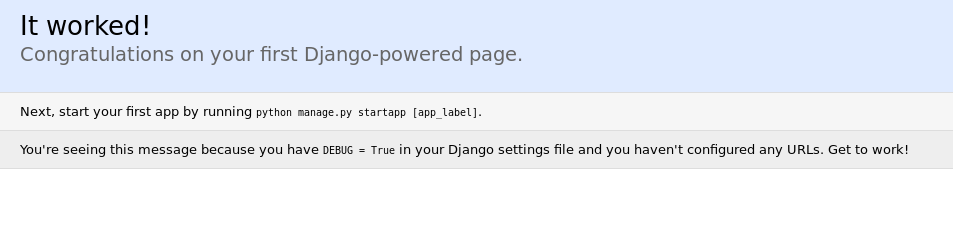
\includegraphics[width=0.7\textwidth]{img/djangook}
\caption{¡Hola mundo! en Django}
\label{djangook}
\end{figure}

El comando \texttt{runserver} ejecuta un servidor de desarrollo escrito en Python. Gracias a esto, el desarrollador puede centrarse en desarrollar la aplicación sin tener que estar lidiando con la configuración de un servidor de producción. Ahora bien, este servidor sólo debe usarse para desarrollo. Una ventaja de este servidor es que se reinicia sólo cuando se modifica el código Python. Una comodidad más para el programador.

\section{Creando la aplicación de horarios}
Una vez tenemos nuestro proyecto creado, es hora de crear la aplicación que se encargará de comunicarse con el módulo Python que hace los horarios. El lector puede preguntarse, ¿cuál es la diferencia entre una app y un proyecto? Una app debe implementar una funcionalidad pequeña (por ejemplo, crear un horario) mientras que un proyecto encapsula varias apps bajo una determinada configuración. Sí, una app \texttt{Django} se puede usar en varios proyectos sin ningún problema.

Al igual que para crear el proyecto, \texttt{Django} ofrece un comando para crear apps:

\begin{minted}{shell-session}
$ python manage.py startapp timetables
\end{minted}

Se puede crear la app en cualquier directorio, aunque por sencillez, yo la creé justo en el mismo directorio que \texttt{manage.py}. Al crear la app, \texttt{Django} crea automáticamente la siguiente estructura de directorios de la \hyperref[djangoappfolders]{Figura \ref*{djangoappfolders}}.

\begin{figure}
\centering
\scalebox{.7}{% Graphic for TeX using PGF
% Title: /home/marta/Diagrama2.dia
% Creator: Dia v0.97.3
% CreationDate: Thu Sep  7 23:06:01 2017
% For: marta
% \usepackage{tikz}
% The following commands are not supported in PSTricks at present
% We define them conditionally, so when they are implemented,
% this pgf file will use them.
\ifx\du\undefined
  \newlength{\du}
\fi
\setlength{\du}{15\unitlength}
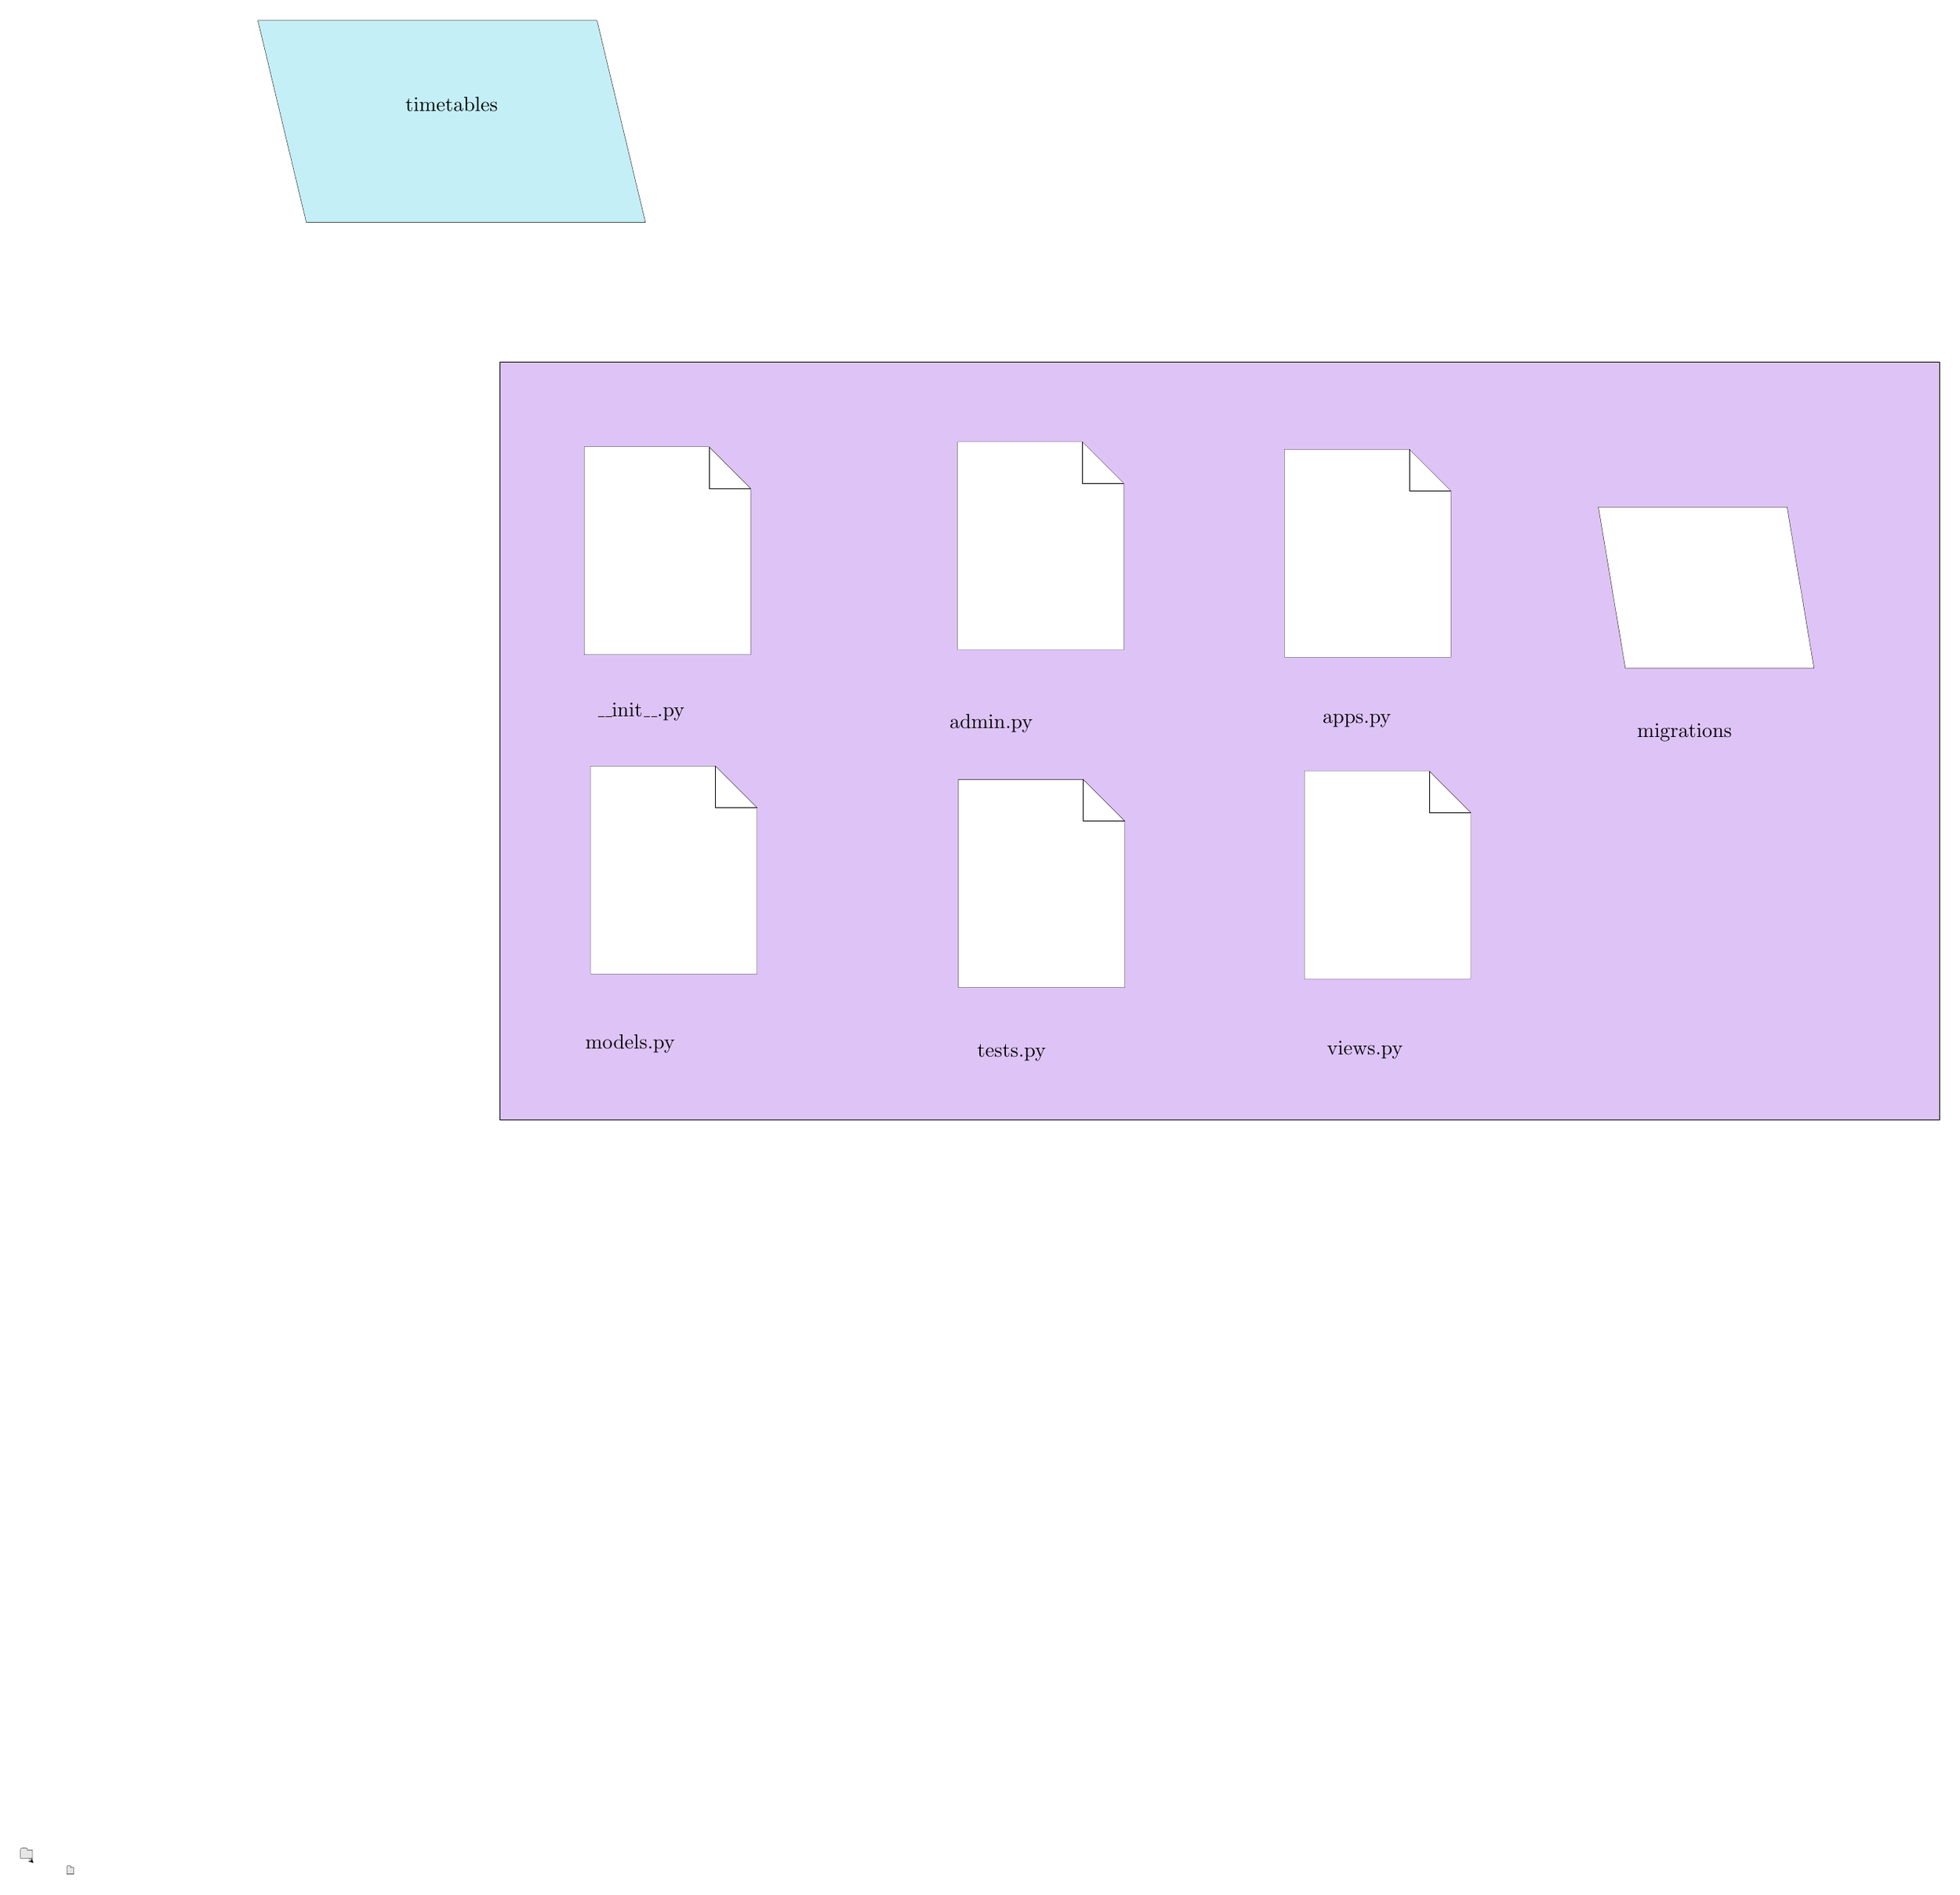
\begin{tikzpicture}
\pgftransformxscale{1.000000}
\pgftransformyscale{-1.000000}
\definecolor{dialinecolor}{rgb}{0.000000, 0.000000, 0.000000}
\pgfsetstrokecolor{dialinecolor}
\definecolor{dialinecolor}{rgb}{1.000000, 1.000000, 1.000000}
\pgfsetfillcolor{dialinecolor}
\pgfsetlinewidth{0.100000\du}
\pgfsetdash{}{0pt}
\pgfsetdash{}{0pt}
\pgfsetbuttcap
\pgfsetmiterjoin
\pgfsetlinewidth{0.100000\du}
\pgfsetbuttcap
\pgfsetmiterjoin
\pgfsetdash{}{0pt}
\definecolor{dialinecolor}{rgb}{0.901961, 0.901961, 0.901961}
\pgfsetfillcolor{dialinecolor}
\pgfpathmoveto{\pgfpoint{5.081250\du}{-33.060000\du}}
\pgfpathcurveto{\pgfpoint{5.081250\du}{-34.050000\du}}{\pgfpoint{5.081250\du}{-34.050000\du}}{\pgfpoint{5.912500\du}{-34.050000\du}}
\pgfpathcurveto{\pgfpoint{6.743750\du}{-34.050000\du}}{\pgfpoint{6.743750\du}{-34.050000\du}}{\pgfpoint{7.575000\du}{-34.050000\du}}
\pgfpathcurveto{\pgfpoint{8.406250\du}{-34.050000\du}}{\pgfpoint{8.406250\du}{-34.050000\du}}{\pgfpoint{8.406250\du}{-33.060000\du}}
\pgfpathcurveto{\pgfpoint{8.406250\du}{-33.060000\du}}{\pgfpoint{10.900000\du}{-33.060000\du}}{\pgfpoint{10.900000\du}{-33.060000\du}}
\pgfpathcurveto{\pgfpoint{10.900000\du}{-33.060000\du}}{\pgfpoint{10.900000\du}{-29.100000\du}}{\pgfpoint{10.900000\du}{-29.100000\du}}
\pgfpathcurveto{\pgfpoint{10.900000\du}{-29.100000\du}}{\pgfpoint{5.081250\du}{-29.100000\du}}{\pgfpoint{5.081250\du}{-29.100000\du}}
\pgfpathcurveto{\pgfpoint{5.081250\du}{-29.100000\du}}{\pgfpoint{5.081250\du}{-32.069999\du}}{\pgfpoint{5.081250\du}{-33.060000\du}}
\pgfusepath{fill}
\definecolor{dialinecolor}{rgb}{0.000000, 0.000000, 0.000000}
\pgfsetstrokecolor{dialinecolor}
\pgfpathmoveto{\pgfpoint{5.081250\du}{-33.060000\du}}
\pgfpathcurveto{\pgfpoint{5.081250\du}{-34.050000\du}}{\pgfpoint{5.081250\du}{-34.050000\du}}{\pgfpoint{5.912500\du}{-34.050000\du}}
\pgfpathcurveto{\pgfpoint{6.743750\du}{-34.050000\du}}{\pgfpoint{6.743750\du}{-34.050000\du}}{\pgfpoint{7.575000\du}{-34.050000\du}}
\pgfpathcurveto{\pgfpoint{8.406250\du}{-34.050000\du}}{\pgfpoint{8.406250\du}{-34.050000\du}}{\pgfpoint{8.406250\du}{-33.060000\du}}
\pgfpathcurveto{\pgfpoint{8.406250\du}{-33.060000\du}}{\pgfpoint{10.900000\du}{-33.060000\du}}{\pgfpoint{10.900000\du}{-33.060000\du}}
\pgfpathcurveto{\pgfpoint{10.900000\du}{-33.060000\du}}{\pgfpoint{10.900000\du}{-29.100000\du}}{\pgfpoint{10.900000\du}{-29.100000\du}}
\pgfpathcurveto{\pgfpoint{10.900000\du}{-29.100000\du}}{\pgfpoint{5.081250\du}{-29.100000\du}}{\pgfpoint{5.081250\du}{-29.100000\du}}
\pgfpathcurveto{\pgfpoint{5.081250\du}{-29.100000\du}}{\pgfpoint{5.081250\du}{-32.069999\du}}{\pgfpoint{5.081250\du}{-33.060000\du}}
\pgfusepath{stroke}
\pgfsetlinewidth{0.010000\du}
\pgfsetbuttcap
\pgfsetmiterjoin
\pgfsetdash{}{0pt}
\definecolor{dialinecolor}{rgb}{0.000000, 0.000000, 0.000000}
\pgfsetstrokecolor{dialinecolor}
\pgfpathmoveto{\pgfpoint{5.081250\du}{-33.060000\du}}
\pgfpathcurveto{\pgfpoint{5.081250\du}{-34.050000\du}}{\pgfpoint{5.081250\du}{-34.050000\du}}{\pgfpoint{5.912500\du}{-34.050000\du}}
\pgfpathcurveto{\pgfpoint{6.743750\du}{-34.050000\du}}{\pgfpoint{6.743750\du}{-34.050000\du}}{\pgfpoint{7.575000\du}{-34.050000\du}}
\pgfpathcurveto{\pgfpoint{8.406250\du}{-34.050000\du}}{\pgfpoint{8.406250\du}{-34.050000\du}}{\pgfpoint{8.406250\du}{-33.060000\du}}
\pgfpathcurveto{\pgfpoint{8.406250\du}{-33.060000\du}}{\pgfpoint{10.900000\du}{-33.060000\du}}{\pgfpoint{10.900000\du}{-33.060000\du}}
\pgfpathcurveto{\pgfpoint{10.900000\du}{-33.060000\du}}{\pgfpoint{10.900000\du}{-29.100000\du}}{\pgfpoint{10.900000\du}{-29.100000\du}}
\pgfpathcurveto{\pgfpoint{10.900000\du}{-29.100000\du}}{\pgfpoint{5.081250\du}{-29.100000\du}}{\pgfpoint{5.081250\du}{-29.100000\du}}
\pgfpathcurveto{\pgfpoint{5.081250\du}{-29.100000\du}}{\pgfpoint{5.081250\du}{-32.069999\du}}{\pgfpoint{5.081250\du}{-33.060000\du}}
\pgfusepath{stroke}
\pgfsetlinewidth{0.100000\du}
\pgfsetbuttcap
\pgfsetmiterjoin
\pgfsetdash{}{0pt}
\definecolor{dialinecolor}{rgb}{0.768627, 0.937255, 0.964706}
\pgfsetfillcolor{dialinecolor}
\fill (5.081250\du,-29.100000\du)--(4.250000\du,-32.564999\du)--(10.068750\du,-32.564999\du)--(10.900000\du,-29.100000\du)--cycle;
\definecolor{dialinecolor}{rgb}{0.000000, 0.000000, 0.000000}
\pgfsetstrokecolor{dialinecolor}
\draw (5.081250\du,-29.100000\du)--(4.250000\du,-32.564999\du)--(10.068750\du,-32.564999\du)--(10.900000\du,-29.100000\du)--cycle;
\pgfsetlinewidth{0.010000\du}
\pgfsetbuttcap
\pgfsetmiterjoin
\pgfsetdash{}{0pt}
\definecolor{dialinecolor}{rgb}{0.000000, 0.000000, 0.000000}
\pgfsetstrokecolor{dialinecolor}
\draw (5.081250\du,-29.100000\du)--(4.250000\du,-32.564999\du)--(10.068750\du,-32.564999\du)--(10.900000\du,-29.100000\du)--cycle;
% setfont left to latex
\definecolor{dialinecolor}{rgb}{0.000000, 0.000000, 0.000000}
\pgfsetstrokecolor{dialinecolor}
\node at (7.575000\du,-31.127500\du){timetables};
\pgfsetlinewidth{0.100000\du}
\pgfsetdash{}{0pt}
\pgfsetdash{}{0pt}
\pgfsetmiterjoin
\definecolor{dialinecolor}{rgb}{0.870588, 0.768627, 0.964706}
\pgfsetfillcolor{dialinecolor}
\fill (8.400000\du,-26.700000\du)--(8.400000\du,-13.700000\du)--(33.100000\du,-13.700000\du)--(33.100000\du,-26.700000\du)--cycle;
\definecolor{dialinecolor}{rgb}{0.000000, 0.000000, 0.000000}
\pgfsetstrokecolor{dialinecolor}
\draw (8.400000\du,-26.700000\du)--(8.400000\du,-13.700000\du)--(33.100000\du,-13.700000\du)--(33.100000\du,-26.700000\du)--cycle;
\pgfsetlinewidth{0.100000\du}
\pgfsetdash{}{0pt}
\pgfsetdash{}{0pt}
\pgfsetbuttcap
{
\definecolor{dialinecolor}{rgb}{0.000000, 0.000000, 0.000000}
\pgfsetfillcolor{dialinecolor}
% was here!!!
\pgfsetarrowsend{stealth}
\definecolor{dialinecolor}{rgb}{0.000000, 0.000000, 0.000000}
\pgfsetstrokecolor{dialinecolor}
\pgfpathmoveto{\pgfpoint{9.331398\du}{-29.051534\du}}
\pgfpatharc{140}{135}{34.537577\du and 34.537577\du}
\pgfusepath{stroke}
}
\pgfsetlinewidth{0.100000\du}
\pgfsetdash{}{0pt}
\pgfsetdash{}{0pt}
\pgfsetbuttcap
\pgfsetmiterjoin
\pgfsetlinewidth{0.100000\du}
\pgfsetbuttcap
\pgfsetmiterjoin
\pgfsetdash{}{0pt}
\definecolor{dialinecolor}{rgb}{1.000000, 1.000000, 1.000000}
\pgfsetfillcolor{dialinecolor}
\fill (9.850000\du,-25.250000\du)--(11.991250\du,-25.250000\du)--(12.705000\du,-24.536250\du)--(12.705000\du,-21.681250\du)--(9.850000\du,-21.681250\du)--cycle;
\definecolor{dialinecolor}{rgb}{0.000000, 0.000000, 0.000000}
\pgfsetstrokecolor{dialinecolor}
\draw (9.850000\du,-25.250000\du)--(11.991250\du,-25.250000\du)--(12.705000\du,-24.536250\du)--(12.705000\du,-21.681250\du)--(9.850000\du,-21.681250\du)--cycle;
\pgfsetbuttcap
\pgfsetmiterjoin
\pgfsetdash{}{0pt}
\definecolor{dialinecolor}{rgb}{0.000000, 0.000000, 0.000000}
\pgfsetstrokecolor{dialinecolor}
\draw (11.991250\du,-25.250000\du)--(11.991250\du,-24.536250\du)--(12.705000\du,-24.536250\du)--(12.705000\du,-24.536250\du);
% setfont left to latex
\definecolor{dialinecolor}{rgb}{0.000000, 0.000000, 0.000000}
\pgfsetstrokecolor{dialinecolor}
\node[anchor=west] at (9.950000\du,-20.700000\du){\_\_init\_\_.py};
\pgfsetlinewidth{0.100000\du}
\pgfsetdash{}{0pt}
\pgfsetdash{}{0pt}
\pgfsetbuttcap
\pgfsetmiterjoin
\pgfsetlinewidth{0.100000\du}
\pgfsetbuttcap
\pgfsetmiterjoin
\pgfsetdash{}{0pt}
\definecolor{dialinecolor}{rgb}{1.000000, 1.000000, 1.000000}
\pgfsetfillcolor{dialinecolor}
\fill (9.960000\du,-19.770000\du)--(12.101250\du,-19.770000\du)--(12.815000\du,-19.056250\du)--(12.815000\du,-16.201250\du)--(9.960000\du,-16.201250\du)--cycle;
\definecolor{dialinecolor}{rgb}{0.000000, 0.000000, 0.000000}
\pgfsetstrokecolor{dialinecolor}
\draw (9.960000\du,-19.770000\du)--(12.101250\du,-19.770000\du)--(12.815000\du,-19.056250\du)--(12.815000\du,-16.201250\du)--(9.960000\du,-16.201250\du)--cycle;
\pgfsetbuttcap
\pgfsetmiterjoin
\pgfsetdash{}{0pt}
\definecolor{dialinecolor}{rgb}{0.000000, 0.000000, 0.000000}
\pgfsetstrokecolor{dialinecolor}
\draw (12.101250\du,-19.770000\du)--(12.101250\du,-19.056250\du)--(12.815000\du,-19.056250\du)--(12.815000\du,-19.056250\du);
% setfont left to latex
\definecolor{dialinecolor}{rgb}{0.000000, 0.000000, 0.000000}
\pgfsetstrokecolor{dialinecolor}
\node[anchor=west] at (9.750000\du,-15.000000\du){models.py};
\pgfsetlinewidth{0.100000\du}
\pgfsetdash{}{0pt}
\pgfsetdash{}{0pt}
\pgfsetbuttcap
\pgfsetmiterjoin
\pgfsetlinewidth{0.100000\du}
\pgfsetbuttcap
\pgfsetmiterjoin
\pgfsetdash{}{0pt}
\definecolor{dialinecolor}{rgb}{1.000000, 1.000000, 1.000000}
\pgfsetfillcolor{dialinecolor}
\fill (21.865000\du,-25.205000\du)--(24.006250\du,-25.205000\du)--(24.720000\du,-24.491250\du)--(24.720000\du,-21.636250\du)--(21.865000\du,-21.636250\du)--cycle;
\definecolor{dialinecolor}{rgb}{0.000000, 0.000000, 0.000000}
\pgfsetstrokecolor{dialinecolor}
\draw (21.865000\du,-25.205000\du)--(24.006250\du,-25.205000\du)--(24.720000\du,-24.491250\du)--(24.720000\du,-21.636250\du)--(21.865000\du,-21.636250\du)--cycle;
\pgfsetbuttcap
\pgfsetmiterjoin
\pgfsetdash{}{0pt}
\definecolor{dialinecolor}{rgb}{0.000000, 0.000000, 0.000000}
\pgfsetstrokecolor{dialinecolor}
\draw (24.006250\du,-25.205000\du)--(24.006250\du,-24.491250\du)--(24.720000\du,-24.491250\du)--(24.720000\du,-24.491250\du);
% setfont left to latex
\definecolor{dialinecolor}{rgb}{0.000000, 0.000000, 0.000000}
\pgfsetstrokecolor{dialinecolor}
\node[anchor=west] at (22.400000\du,-20.550000\du){apps.py};
% setfont left to latex
\definecolor{dialinecolor}{rgb}{0.000000, 0.000000, 0.000000}
\pgfsetstrokecolor{dialinecolor}
\node[anchor=west] at (16.000000\du,-20.500000\du){admin.py};
\pgfsetlinewidth{0.100000\du}
\pgfsetdash{}{0pt}
\pgfsetdash{}{0pt}
\pgfsetbuttcap
\pgfsetmiterjoin
\pgfsetlinewidth{0.100000\du}
\pgfsetbuttcap
\pgfsetmiterjoin
\pgfsetdash{}{0pt}
\definecolor{dialinecolor}{rgb}{1.000000, 1.000000, 1.000000}
\pgfsetfillcolor{dialinecolor}
\fill (16.255000\du,-25.335000\du)--(18.396250\du,-25.335000\du)--(19.110000\du,-24.621250\du)--(19.110000\du,-21.766250\du)--(16.255000\du,-21.766250\du)--cycle;
\definecolor{dialinecolor}{rgb}{0.000000, 0.000000, 0.000000}
\pgfsetstrokecolor{dialinecolor}
\draw (16.255000\du,-25.335000\du)--(18.396250\du,-25.335000\du)--(19.110000\du,-24.621250\du)--(19.110000\du,-21.766250\du)--(16.255000\du,-21.766250\du)--cycle;
\pgfsetbuttcap
\pgfsetmiterjoin
\pgfsetdash{}{0pt}
\definecolor{dialinecolor}{rgb}{0.000000, 0.000000, 0.000000}
\pgfsetstrokecolor{dialinecolor}
\draw (18.396250\du,-25.335000\du)--(18.396250\du,-24.621250\du)--(19.110000\du,-24.621250\du)--(19.110000\du,-24.621250\du);
\pgfsetlinewidth{0.100000\du}
\pgfsetdash{}{0pt}
\pgfsetdash{}{0pt}
\pgfsetbuttcap
\pgfsetmiterjoin
\pgfsetlinewidth{0.100000\du}
\pgfsetbuttcap
\pgfsetmiterjoin
\pgfsetdash{}{0pt}
\definecolor{dialinecolor}{rgb}{1.000000, 1.000000, 1.000000}
\pgfsetfillcolor{dialinecolor}
\fill (16.270000\du,-19.540000\du)--(18.411250\du,-19.540000\du)--(19.125000\du,-18.826250\du)--(19.125000\du,-15.971250\du)--(16.270000\du,-15.971250\du)--cycle;
\definecolor{dialinecolor}{rgb}{0.000000, 0.000000, 0.000000}
\pgfsetstrokecolor{dialinecolor}
\draw (16.270000\du,-19.540000\du)--(18.411250\du,-19.540000\du)--(19.125000\du,-18.826250\du)--(19.125000\du,-15.971250\du)--(16.270000\du,-15.971250\du)--cycle;
\pgfsetbuttcap
\pgfsetmiterjoin
\pgfsetdash{}{0pt}
\definecolor{dialinecolor}{rgb}{0.000000, 0.000000, 0.000000}
\pgfsetstrokecolor{dialinecolor}
\draw (18.411250\du,-19.540000\du)--(18.411250\du,-18.826250\du)--(19.125000\du,-18.826250\du)--(19.125000\du,-18.826250\du);
% setfont left to latex
\definecolor{dialinecolor}{rgb}{0.000000, 0.000000, 0.000000}
\pgfsetstrokecolor{dialinecolor}
\node[anchor=west] at (16.475000\du,-14.850000\du){tests.py};
\pgfsetlinewidth{0.100000\du}
\pgfsetdash{}{0pt}
\pgfsetdash{}{0pt}
\pgfsetbuttcap
\pgfsetmiterjoin
\pgfsetlinewidth{0.100000\du}
\pgfsetbuttcap
\pgfsetmiterjoin
\pgfsetdash{}{0pt}
\definecolor{dialinecolor}{rgb}{1.000000, 1.000000, 1.000000}
\pgfsetfillcolor{dialinecolor}
\fill (22.205000\du,-19.685000\du)--(24.346250\du,-19.685000\du)--(25.060000\du,-18.971250\du)--(25.060000\du,-16.116250\du)--(22.205000\du,-16.116250\du)--cycle;
\definecolor{dialinecolor}{rgb}{0.000000, 0.000000, 0.000000}
\pgfsetstrokecolor{dialinecolor}
\draw (22.205000\du,-19.685000\du)--(24.346250\du,-19.685000\du)--(25.060000\du,-18.971250\du)--(25.060000\du,-16.116250\du)--(22.205000\du,-16.116250\du)--cycle;
\pgfsetbuttcap
\pgfsetmiterjoin
\pgfsetdash{}{0pt}
\definecolor{dialinecolor}{rgb}{0.000000, 0.000000, 0.000000}
\pgfsetstrokecolor{dialinecolor}
\draw (24.346250\du,-19.685000\du)--(24.346250\du,-18.971250\du)--(25.060000\du,-18.971250\du)--(25.060000\du,-18.971250\du);
% setfont left to latex
\definecolor{dialinecolor}{rgb}{0.000000, 0.000000, 0.000000}
\pgfsetstrokecolor{dialinecolor}
\node[anchor=west] at (22.475000\du,-14.900000\du){views.py};
\pgfsetlinewidth{0.100000\du}
\pgfsetdash{}{0pt}
\pgfsetdash{}{0pt}
\pgfsetbuttcap
\pgfsetmiterjoin
\pgfsetlinewidth{0.100000\du}
\pgfsetbuttcap
\pgfsetmiterjoin
\pgfsetdash{}{0pt}
\definecolor{dialinecolor}{rgb}{0.901961, 0.901961, 0.901961}
\pgfsetfillcolor{dialinecolor}
\pgfpathmoveto{\pgfpoint{27.712500\du}{-24.610000\du}}
\pgfpathcurveto{\pgfpoint{27.712500\du}{-25.400000\du}}{\pgfpoint{27.712500\du}{-25.400000\du}}{\pgfpoint{28.175000\du}{-25.400000\du}}
\pgfpathcurveto{\pgfpoint{28.637500\du}{-25.400000\du}}{\pgfpoint{28.637500\du}{-25.400000\du}}{\pgfpoint{29.100000\du}{-25.400000\du}}
\pgfpathcurveto{\pgfpoint{29.562500\du}{-25.400000\du}}{\pgfpoint{29.562500\du}{-25.400000\du}}{\pgfpoint{29.562500\du}{-24.610000\du}}
\pgfpathcurveto{\pgfpoint{29.562500\du}{-24.610000\du}}{\pgfpoint{30.950000\du}{-24.610000\du}}{\pgfpoint{30.950000\du}{-24.610000\du}}
\pgfpathcurveto{\pgfpoint{30.950000\du}{-24.610000\du}}{\pgfpoint{30.950000\du}{-21.450000\du}}{\pgfpoint{30.950000\du}{-21.450000\du}}
\pgfpathcurveto{\pgfpoint{30.950000\du}{-21.450000\du}}{\pgfpoint{27.712500\du}{-21.450000\du}}{\pgfpoint{27.712500\du}{-21.450000\du}}
\pgfpathcurveto{\pgfpoint{27.712500\du}{-21.450000\du}}{\pgfpoint{27.712500\du}{-23.820000\du}}{\pgfpoint{27.712500\du}{-24.610000\du}}
\pgfusepath{fill}
\definecolor{dialinecolor}{rgb}{0.000000, 0.000000, 0.000000}
\pgfsetstrokecolor{dialinecolor}
\pgfpathmoveto{\pgfpoint{27.712500\du}{-24.610000\du}}
\pgfpathcurveto{\pgfpoint{27.712500\du}{-25.400000\du}}{\pgfpoint{27.712500\du}{-25.400000\du}}{\pgfpoint{28.175000\du}{-25.400000\du}}
\pgfpathcurveto{\pgfpoint{28.637500\du}{-25.400000\du}}{\pgfpoint{28.637500\du}{-25.400000\du}}{\pgfpoint{29.100000\du}{-25.400000\du}}
\pgfpathcurveto{\pgfpoint{29.562500\du}{-25.400000\du}}{\pgfpoint{29.562500\du}{-25.400000\du}}{\pgfpoint{29.562500\du}{-24.610000\du}}
\pgfpathcurveto{\pgfpoint{29.562500\du}{-24.610000\du}}{\pgfpoint{30.950000\du}{-24.610000\du}}{\pgfpoint{30.950000\du}{-24.610000\du}}
\pgfpathcurveto{\pgfpoint{30.950000\du}{-24.610000\du}}{\pgfpoint{30.950000\du}{-21.450000\du}}{\pgfpoint{30.950000\du}{-21.450000\du}}
\pgfpathcurveto{\pgfpoint{30.950000\du}{-21.450000\du}}{\pgfpoint{27.712500\du}{-21.450000\du}}{\pgfpoint{27.712500\du}{-21.450000\du}}
\pgfpathcurveto{\pgfpoint{27.712500\du}{-21.450000\du}}{\pgfpoint{27.712500\du}{-23.820000\du}}{\pgfpoint{27.712500\du}{-24.610000\du}}
\pgfusepath{stroke}
\pgfsetlinewidth{0.010000\du}
\pgfsetbuttcap
\pgfsetmiterjoin
\pgfsetdash{}{0pt}
\definecolor{dialinecolor}{rgb}{0.000000, 0.000000, 0.000000}
\pgfsetstrokecolor{dialinecolor}
\pgfpathmoveto{\pgfpoint{27.712500\du}{-24.610000\du}}
\pgfpathcurveto{\pgfpoint{27.712500\du}{-25.400000\du}}{\pgfpoint{27.712500\du}{-25.400000\du}}{\pgfpoint{28.175000\du}{-25.400000\du}}
\pgfpathcurveto{\pgfpoint{28.637500\du}{-25.400000\du}}{\pgfpoint{28.637500\du}{-25.400000\du}}{\pgfpoint{29.100000\du}{-25.400000\du}}
\pgfpathcurveto{\pgfpoint{29.562500\du}{-25.400000\du}}{\pgfpoint{29.562500\du}{-25.400000\du}}{\pgfpoint{29.562500\du}{-24.610000\du}}
\pgfpathcurveto{\pgfpoint{29.562500\du}{-24.610000\du}}{\pgfpoint{30.950000\du}{-24.610000\du}}{\pgfpoint{30.950000\du}{-24.610000\du}}
\pgfpathcurveto{\pgfpoint{30.950000\du}{-24.610000\du}}{\pgfpoint{30.950000\du}{-21.450000\du}}{\pgfpoint{30.950000\du}{-21.450000\du}}
\pgfpathcurveto{\pgfpoint{30.950000\du}{-21.450000\du}}{\pgfpoint{27.712500\du}{-21.450000\du}}{\pgfpoint{27.712500\du}{-21.450000\du}}
\pgfpathcurveto{\pgfpoint{27.712500\du}{-21.450000\du}}{\pgfpoint{27.712500\du}{-23.820000\du}}{\pgfpoint{27.712500\du}{-24.610000\du}}
\pgfusepath{stroke}
\pgfsetlinewidth{0.100000\du}
\pgfsetbuttcap
\pgfsetmiterjoin
\pgfsetdash{}{0pt}
\definecolor{dialinecolor}{rgb}{1.000000, 1.000000, 1.000000}
\pgfsetfillcolor{dialinecolor}
\fill (27.712500\du,-21.450000\du)--(27.250000\du,-24.215000\du)--(30.487500\du,-24.215000\du)--(30.950000\du,-21.450000\du)--cycle;
\definecolor{dialinecolor}{rgb}{0.000000, 0.000000, 0.000000}
\pgfsetstrokecolor{dialinecolor}
\draw (27.712500\du,-21.450000\du)--(27.250000\du,-24.215000\du)--(30.487500\du,-24.215000\du)--(30.950000\du,-21.450000\du)--cycle;
\pgfsetlinewidth{0.010000\du}
\pgfsetbuttcap
\pgfsetmiterjoin
\pgfsetdash{}{0pt}
\definecolor{dialinecolor}{rgb}{0.000000, 0.000000, 0.000000}
\pgfsetstrokecolor{dialinecolor}
\draw (27.712500\du,-21.450000\du)--(27.250000\du,-24.215000\du)--(30.487500\du,-24.215000\du)--(30.950000\du,-21.450000\du)--cycle;
% setfont left to latex
\definecolor{dialinecolor}{rgb}{0.000000, 0.000000, 0.000000}
\pgfsetstrokecolor{dialinecolor}
\node at (29.100000\du,-23.027500\du){};
% setfont left to latex
\definecolor{dialinecolor}{rgb}{0.000000, 0.000000, 0.000000}
\pgfsetstrokecolor{dialinecolor}
\node[anchor=west] at (27.800000\du,-20.350000\du){migrations};
\end{tikzpicture}
}
\caption{Estructura de directorios inicial de una aplicación Django}
\label{djangoappfolders}
\end{figure}

Una vez hemos creado nuestra app, es muy importante añadirla a la configuración de nuestro proyecto y que éste sepa que nuestra app existe. Para ello, sólo tenemos que modificar el fichero \texttt{djangoapp/settings.py} y añadir nuestra app a la lista \texttt{INSTALLED\_APPS}:

\newpage
\begin{minted}{python}
INSTALLED_APPS = [
    'timetables.apps.TimetablesConfig',
    'django.contrib.admin',
    'django.contrib.auth',
    'django.contrib.contenttypes',
    'django.contrib.sessions',
    'django.contrib.messages',
    'django.contrib.staticfiles',
]
\end{minted}

Ya lo tenemos todo preparado para empezar a trabajar en nuestra app.

\subsection{Definiendo los modelos}
\begin{figure}
\centering
\scalebox{.7}{% Graphic for TeX using PGF
% Title: /home/marta/Diagrama3.dia
% Creator: Dia v0.97.3
% CreationDate: Thu Sep  7 23:36:28 2017
% For: marta
% \usepackage{tikz}
% The following commands are not supported in PSTricks at present
% We define them conditionally, so when they are implemented,
% this pgf file will use them.
\ifx\du\undefined
  \newlength{\du}
\fi
\setlength{\du}{15\unitlength}
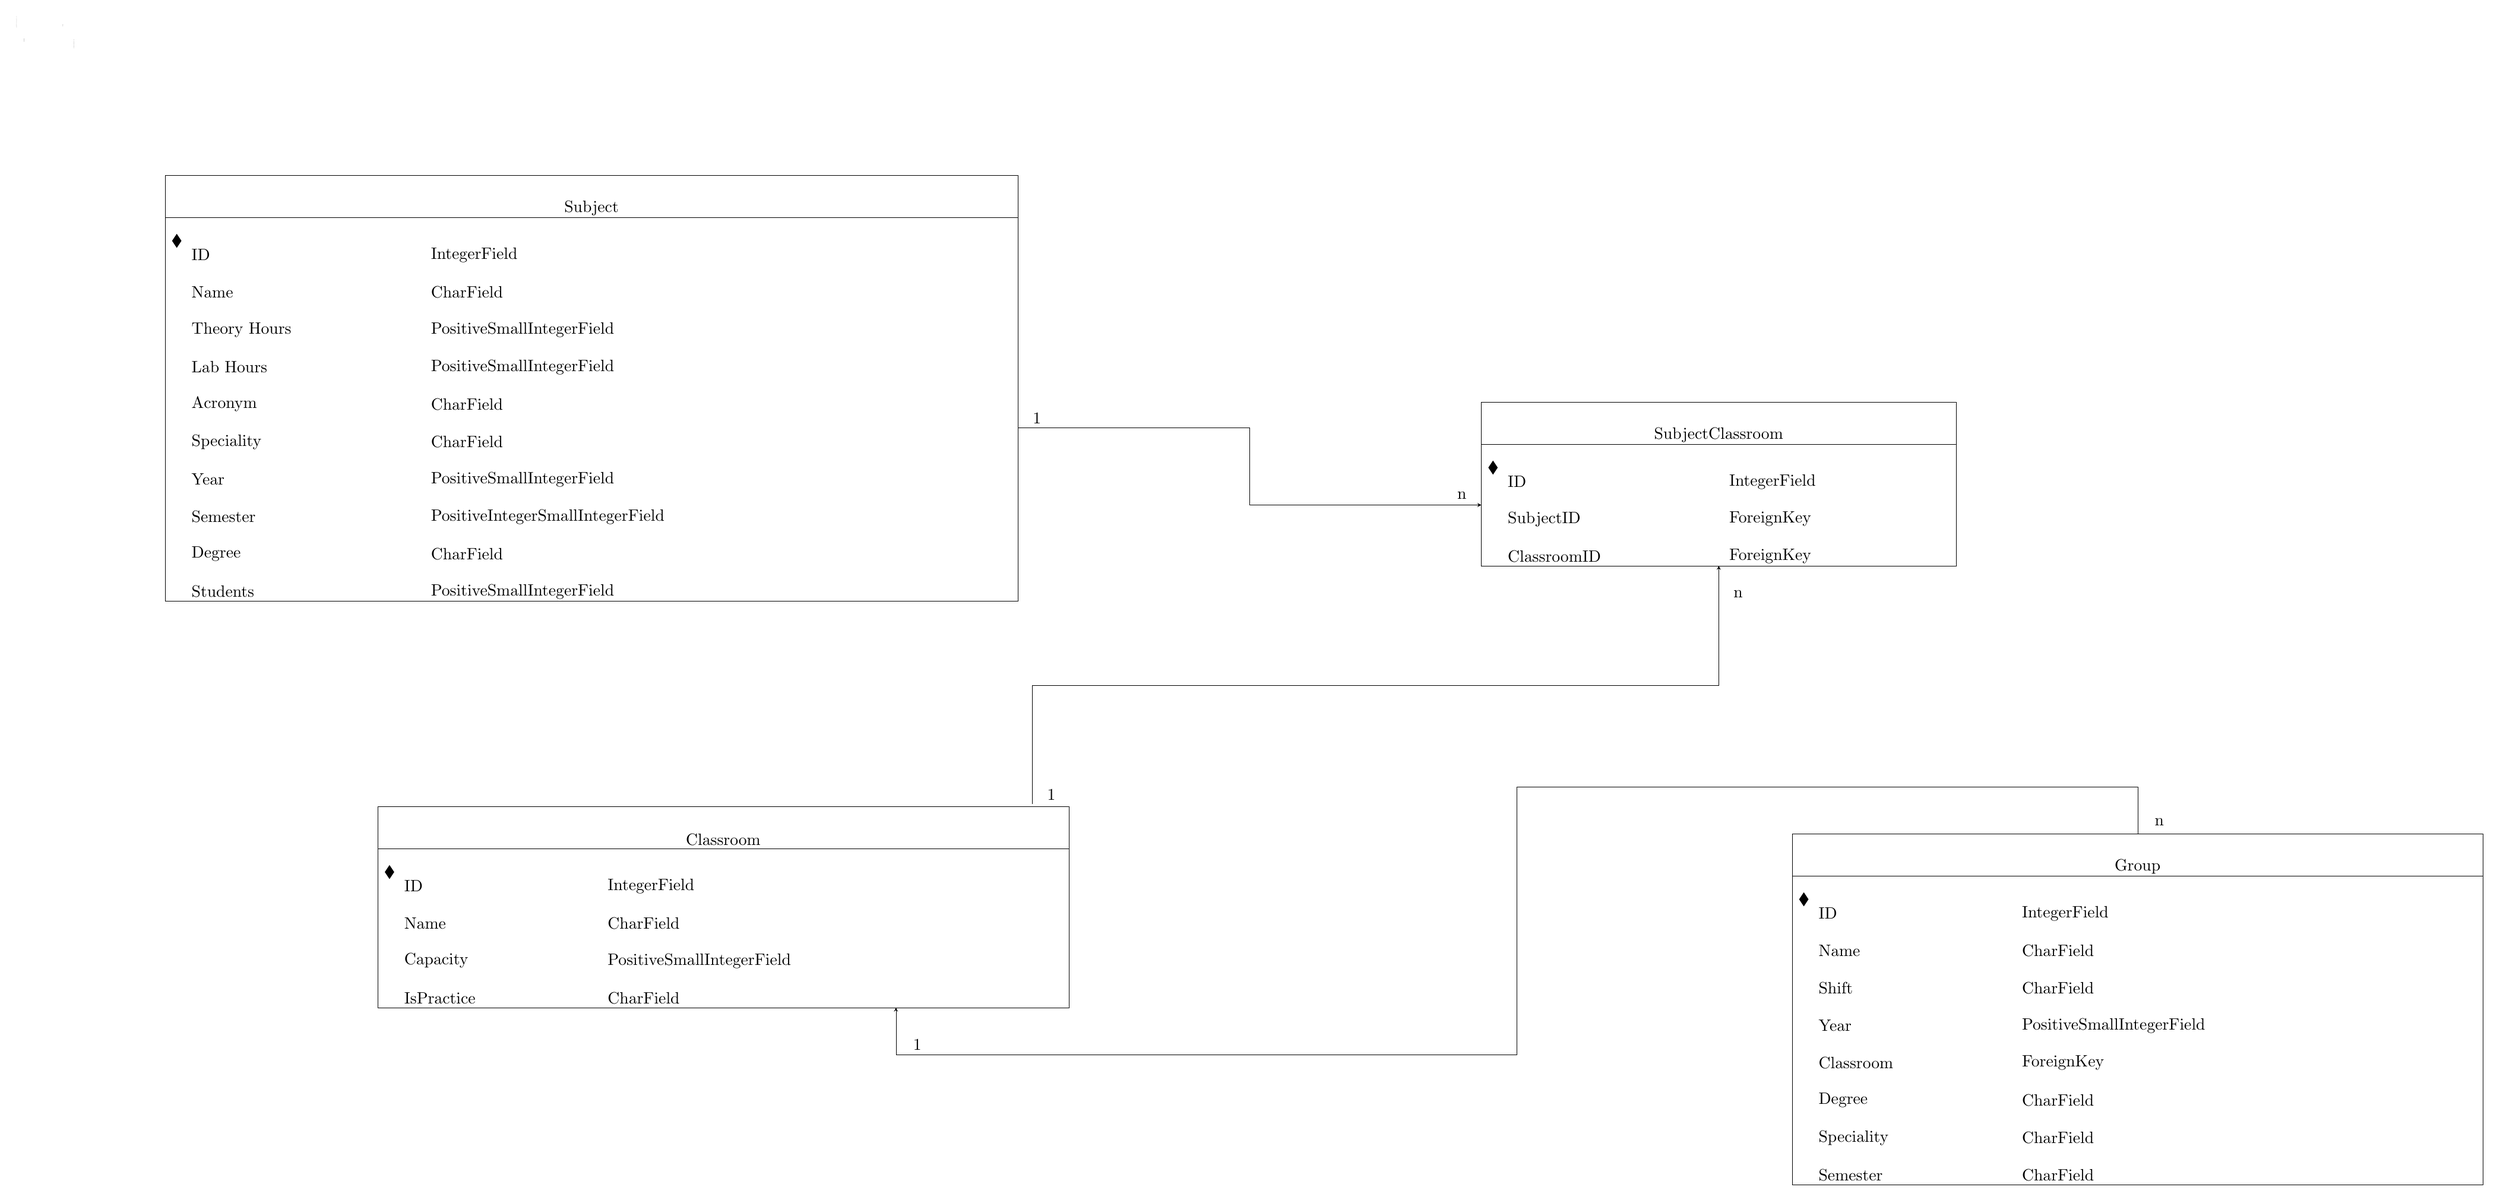
\begin{tikzpicture}
\pgftransformxscale{1.000000}
\pgftransformyscale{-1.000000}
\definecolor{dialinecolor}{rgb}{0.000000, 0.000000, 0.000000}
\pgfsetstrokecolor{dialinecolor}
\definecolor{dialinecolor}{rgb}{1.000000, 1.000000, 1.000000}
\pgfsetfillcolor{dialinecolor}
\pgfsetlinewidth{0.100000\du}
\pgfsetdash{}{0pt}
\definecolor{dialinecolor}{rgb}{1.000000, 1.000000, 1.000000}
\pgfsetfillcolor{dialinecolor}
\fill (3.300000\du,3.600000\du)--(3.300000\du,4.500000\du)--(21.540000\du,4.500000\du)--(21.540000\du,3.600000\du)--cycle;
\definecolor{dialinecolor}{rgb}{0.000000, 0.000000, 0.000000}
\pgfsetstrokecolor{dialinecolor}
\draw (3.300000\du,3.600000\du)--(3.300000\du,4.500000\du)--(21.540000\du,4.500000\du)--(21.540000\du,3.600000\du)--cycle;
% setfont left to latex
\definecolor{dialinecolor}{rgb}{0.000000, 0.000000, 0.000000}
\pgfsetstrokecolor{dialinecolor}
\node at (12.420000\du,4.300000\du){Subject};
\definecolor{dialinecolor}{rgb}{1.000000, 1.000000, 1.000000}
\pgfsetfillcolor{dialinecolor}
\fill (3.300000\du,4.500000\du)--(3.300000\du,12.700000\du)--(21.540000\du,12.700000\du)--(21.540000\du,4.500000\du)--cycle;
\definecolor{dialinecolor}{rgb}{0.000000, 0.000000, 0.000000}
\pgfsetstrokecolor{dialinecolor}
\draw (3.300000\du,4.500000\du)--(3.300000\du,12.700000\du)--(21.540000\du,12.700000\du)--(21.540000\du,4.500000\du)--cycle;
% setfont left to latex
\pgfsetlinewidth{0.010000\du}
\pgfsetmiterjoin
\definecolor{dialinecolor}{rgb}{0.000000, 0.000000, 0.000000}
\pgfsetfillcolor{dialinecolor}
\fill (3.450000\du,5.000000\du)--(3.550000\du,5.150000\du)--(3.650000\du,5.000000\du)--(3.550000\du,4.850000\du)--cycle;
\definecolor{dialinecolor}{rgb}{0.000000, 0.000000, 0.000000}
\pgfsetstrokecolor{dialinecolor}
\node[anchor=west] at (3.750000\du,5.300000\du){ID};
\definecolor{dialinecolor}{rgb}{0.000000, 0.000000, 0.000000}
\pgfsetstrokecolor{dialinecolor}
\node[anchor=west] at (8.870000\du,5.300000\du){IntegerField};
% setfont left to latex
\pgfsetlinewidth{0.010000\du}
\definecolor{dialinecolor}{rgb}{0.000000, 0.000000, 0.000000}
\pgfsetfillcolor{dialinecolor}
\pgfpathellipse{\pgfpoint{3.550000\du}{5.800000\du}}{\pgfpoint{0.100000\du}{0\du}}{\pgfpoint{0\du}{0.100000\du}}
\pgfusepath{fill}
\definecolor{dialinecolor}{rgb}{0.000000, 0.000000, 0.000000}
\pgfsetstrokecolor{dialinecolor}
\node[anchor=west] at (3.750000\du,6.100000\du){Name};
\definecolor{dialinecolor}{rgb}{0.000000, 0.000000, 0.000000}
\pgfsetstrokecolor{dialinecolor}
\node[anchor=west] at (8.870000\du,6.100000\du){CharField};
% setfont left to latex
\pgfsetlinewidth{0.010000\du}
\definecolor{dialinecolor}{rgb}{0.000000, 0.000000, 0.000000}
\pgfsetfillcolor{dialinecolor}
\pgfpathellipse{\pgfpoint{3.550000\du}{6.600000\du}}{\pgfpoint{0.100000\du}{0\du}}{\pgfpoint{0\du}{0.100000\du}}
\pgfusepath{fill}
\definecolor{dialinecolor}{rgb}{0.000000, 0.000000, 0.000000}
\pgfsetstrokecolor{dialinecolor}
\node[anchor=west] at (3.750000\du,6.900000\du){Theory Hours};
\definecolor{dialinecolor}{rgb}{0.000000, 0.000000, 0.000000}
\pgfsetstrokecolor{dialinecolor}
\node[anchor=west] at (8.870000\du,6.900000\du){PositiveSmallIntegerField};
% setfont left to latex
\pgfsetlinewidth{0.010000\du}
\definecolor{dialinecolor}{rgb}{0.000000, 0.000000, 0.000000}
\pgfsetfillcolor{dialinecolor}
\pgfpathellipse{\pgfpoint{3.550000\du}{7.400000\du}}{\pgfpoint{0.100000\du}{0\du}}{\pgfpoint{0\du}{0.100000\du}}
\pgfusepath{fill}
\definecolor{dialinecolor}{rgb}{0.000000, 0.000000, 0.000000}
\pgfsetstrokecolor{dialinecolor}
\node[anchor=west] at (3.750000\du,7.700000\du){Lab Hours};
\definecolor{dialinecolor}{rgb}{0.000000, 0.000000, 0.000000}
\pgfsetstrokecolor{dialinecolor}
\node[anchor=west] at (8.870000\du,7.700000\du){PositiveSmallIntegerField};
% setfont left to latex
\pgfsetlinewidth{0.010000\du}
\definecolor{dialinecolor}{rgb}{0.000000, 0.000000, 0.000000}
\pgfsetfillcolor{dialinecolor}
\pgfpathellipse{\pgfpoint{3.550000\du}{8.200000\du}}{\pgfpoint{0.100000\du}{0\du}}{\pgfpoint{0\du}{0.100000\du}}
\pgfusepath{fill}
\definecolor{dialinecolor}{rgb}{0.000000, 0.000000, 0.000000}
\pgfsetstrokecolor{dialinecolor}
\node[anchor=west] at (3.750000\du,8.500000\du){Acronym};
\definecolor{dialinecolor}{rgb}{0.000000, 0.000000, 0.000000}
\pgfsetstrokecolor{dialinecolor}
\node[anchor=west] at (8.870000\du,8.500000\du){CharField};
% setfont left to latex
\pgfsetlinewidth{0.010000\du}
\definecolor{dialinecolor}{rgb}{0.000000, 0.000000, 0.000000}
\pgfsetfillcolor{dialinecolor}
\pgfpathellipse{\pgfpoint{3.550000\du}{9.000000\du}}{\pgfpoint{0.100000\du}{0\du}}{\pgfpoint{0\du}{0.100000\du}}
\pgfusepath{fill}
\definecolor{dialinecolor}{rgb}{0.000000, 0.000000, 0.000000}
\pgfsetstrokecolor{dialinecolor}
\node[anchor=west] at (3.750000\du,9.300000\du){Speciality};
\definecolor{dialinecolor}{rgb}{0.000000, 0.000000, 0.000000}
\pgfsetstrokecolor{dialinecolor}
\node[anchor=west] at (8.870000\du,9.300000\du){CharField};
% setfont left to latex
\pgfsetlinewidth{0.010000\du}
\definecolor{dialinecolor}{rgb}{0.000000, 0.000000, 0.000000}
\pgfsetfillcolor{dialinecolor}
\pgfpathellipse{\pgfpoint{3.550000\du}{9.800000\du}}{\pgfpoint{0.100000\du}{0\du}}{\pgfpoint{0\du}{0.100000\du}}
\pgfusepath{fill}
\definecolor{dialinecolor}{rgb}{0.000000, 0.000000, 0.000000}
\pgfsetstrokecolor{dialinecolor}
\node[anchor=west] at (3.750000\du,10.100000\du){Year};
\definecolor{dialinecolor}{rgb}{0.000000, 0.000000, 0.000000}
\pgfsetstrokecolor{dialinecolor}
\node[anchor=west] at (8.870000\du,10.100000\du){PositiveSmallIntegerField};
% setfont left to latex
\pgfsetlinewidth{0.010000\du}
\definecolor{dialinecolor}{rgb}{0.000000, 0.000000, 0.000000}
\pgfsetfillcolor{dialinecolor}
\pgfpathellipse{\pgfpoint{3.550000\du}{10.600000\du}}{\pgfpoint{0.100000\du}{0\du}}{\pgfpoint{0\du}{0.100000\du}}
\pgfusepath{fill}
\definecolor{dialinecolor}{rgb}{0.000000, 0.000000, 0.000000}
\pgfsetstrokecolor{dialinecolor}
\node[anchor=west] at (3.750000\du,10.900000\du){Semester};
\definecolor{dialinecolor}{rgb}{0.000000, 0.000000, 0.000000}
\pgfsetstrokecolor{dialinecolor}
\node[anchor=west] at (8.870000\du,10.900000\du){PositiveIntegerSmallIntegerField};
% setfont left to latex
\pgfsetlinewidth{0.010000\du}
\definecolor{dialinecolor}{rgb}{0.000000, 0.000000, 0.000000}
\pgfsetfillcolor{dialinecolor}
\pgfpathellipse{\pgfpoint{3.550000\du}{11.400000\du}}{\pgfpoint{0.100000\du}{0\du}}{\pgfpoint{0\du}{0.100000\du}}
\pgfusepath{fill}
\definecolor{dialinecolor}{rgb}{0.000000, 0.000000, 0.000000}
\pgfsetstrokecolor{dialinecolor}
\node[anchor=west] at (3.750000\du,11.700000\du){Degree};
\definecolor{dialinecolor}{rgb}{0.000000, 0.000000, 0.000000}
\pgfsetstrokecolor{dialinecolor}
\node[anchor=west] at (8.870000\du,11.700000\du){CharField};
% setfont left to latex
\pgfsetlinewidth{0.010000\du}
\definecolor{dialinecolor}{rgb}{0.000000, 0.000000, 0.000000}
\pgfsetfillcolor{dialinecolor}
\pgfpathellipse{\pgfpoint{3.550000\du}{12.200000\du}}{\pgfpoint{0.100000\du}{0\du}}{\pgfpoint{0\du}{0.100000\du}}
\pgfusepath{fill}
\definecolor{dialinecolor}{rgb}{0.000000, 0.000000, 0.000000}
\pgfsetstrokecolor{dialinecolor}
\node[anchor=west] at (3.750000\du,12.500000\du){Students};
\definecolor{dialinecolor}{rgb}{0.000000, 0.000000, 0.000000}
\pgfsetstrokecolor{dialinecolor}
\node[anchor=west] at (8.870000\du,12.500000\du){PositiveSmallIntegerField};
\pgfsetlinewidth{0.100000\du}
\pgfsetdash{}{0pt}
\definecolor{dialinecolor}{rgb}{1.000000, 1.000000, 1.000000}
\pgfsetfillcolor{dialinecolor}
\fill (7.850000\du,17.100000\du)--(7.850000\du,18.000000\du)--(22.625000\du,18.000000\du)--(22.625000\du,17.100000\du)--cycle;
\definecolor{dialinecolor}{rgb}{0.000000, 0.000000, 0.000000}
\pgfsetstrokecolor{dialinecolor}
\draw (7.850000\du,17.100000\du)--(7.850000\du,18.000000\du)--(22.625000\du,18.000000\du)--(22.625000\du,17.100000\du)--cycle;
% setfont left to latex
\definecolor{dialinecolor}{rgb}{0.000000, 0.000000, 0.000000}
\pgfsetstrokecolor{dialinecolor}
\node at (15.237500\du,17.800000\du){Classroom};
\definecolor{dialinecolor}{rgb}{1.000000, 1.000000, 1.000000}
\pgfsetfillcolor{dialinecolor}
\fill (7.850000\du,18.000000\du)--(7.850000\du,21.400000\du)--(22.625000\du,21.400000\du)--(22.625000\du,18.000000\du)--cycle;
\definecolor{dialinecolor}{rgb}{0.000000, 0.000000, 0.000000}
\pgfsetstrokecolor{dialinecolor}
\draw (7.850000\du,18.000000\du)--(7.850000\du,21.400000\du)--(22.625000\du,21.400000\du)--(22.625000\du,18.000000\du)--cycle;
% setfont left to latex
\pgfsetlinewidth{0.010000\du}
\pgfsetmiterjoin
\definecolor{dialinecolor}{rgb}{0.000000, 0.000000, 0.000000}
\pgfsetfillcolor{dialinecolor}
\fill (8.000000\du,18.500000\du)--(8.100000\du,18.650000\du)--(8.200000\du,18.500000\du)--(8.100000\du,18.350000\du)--cycle;
\definecolor{dialinecolor}{rgb}{0.000000, 0.000000, 0.000000}
\pgfsetstrokecolor{dialinecolor}
\node[anchor=west] at (8.300000\du,18.800000\du){ID};
\definecolor{dialinecolor}{rgb}{0.000000, 0.000000, 0.000000}
\pgfsetstrokecolor{dialinecolor}
\node[anchor=west] at (12.650000\du,18.800000\du){IntegerField};
% setfont left to latex
\pgfsetlinewidth{0.010000\du}
\definecolor{dialinecolor}{rgb}{0.000000, 0.000000, 0.000000}
\pgfsetfillcolor{dialinecolor}
\pgfpathellipse{\pgfpoint{8.100000\du}{19.300000\du}}{\pgfpoint{0.100000\du}{0\du}}{\pgfpoint{0\du}{0.100000\du}}
\pgfusepath{fill}
\definecolor{dialinecolor}{rgb}{0.000000, 0.000000, 0.000000}
\pgfsetstrokecolor{dialinecolor}
\node[anchor=west] at (8.300000\du,19.600000\du){Name};
\definecolor{dialinecolor}{rgb}{0.000000, 0.000000, 0.000000}
\pgfsetstrokecolor{dialinecolor}
\node[anchor=west] at (12.650000\du,19.600000\du){CharField};
% setfont left to latex
\pgfsetlinewidth{0.010000\du}
\definecolor{dialinecolor}{rgb}{0.000000, 0.000000, 0.000000}
\pgfsetfillcolor{dialinecolor}
\pgfpathellipse{\pgfpoint{8.100000\du}{20.100000\du}}{\pgfpoint{0.100000\du}{0\du}}{\pgfpoint{0\du}{0.100000\du}}
\pgfusepath{fill}
\definecolor{dialinecolor}{rgb}{0.000000, 0.000000, 0.000000}
\pgfsetstrokecolor{dialinecolor}
\node[anchor=west] at (8.300000\du,20.400000\du){Capacity};
\definecolor{dialinecolor}{rgb}{0.000000, 0.000000, 0.000000}
\pgfsetstrokecolor{dialinecolor}
\node[anchor=west] at (12.650000\du,20.400000\du){PositiveSmallIntegerField};
% setfont left to latex
\pgfsetlinewidth{0.010000\du}
\definecolor{dialinecolor}{rgb}{0.000000, 0.000000, 0.000000}
\pgfsetfillcolor{dialinecolor}
\pgfpathellipse{\pgfpoint{8.100000\du}{20.900000\du}}{\pgfpoint{0.100000\du}{0\du}}{\pgfpoint{0\du}{0.100000\du}}
\pgfusepath{fill}
\definecolor{dialinecolor}{rgb}{0.000000, 0.000000, 0.000000}
\pgfsetstrokecolor{dialinecolor}
\node[anchor=west] at (8.300000\du,21.200000\du){IsPractice};
\definecolor{dialinecolor}{rgb}{0.000000, 0.000000, 0.000000}
\pgfsetstrokecolor{dialinecolor}
\node[anchor=west] at (12.650000\du,21.200000\du){CharField};
\pgfsetlinewidth{0.100000\du}
\pgfsetdash{}{0pt}
\definecolor{dialinecolor}{rgb}{1.000000, 1.000000, 1.000000}
\pgfsetfillcolor{dialinecolor}
\fill (38.097224\du,17.684124\du)--(38.097224\du,18.584124\du)--(52.872224\du,18.584124\du)--(52.872224\du,17.684124\du)--cycle;
\definecolor{dialinecolor}{rgb}{0.000000, 0.000000, 0.000000}
\pgfsetstrokecolor{dialinecolor}
\draw (38.097224\du,17.684124\du)--(38.097224\du,18.584124\du)--(52.872224\du,18.584124\du)--(52.872224\du,17.684124\du)--cycle;
% setfont left to latex
\definecolor{dialinecolor}{rgb}{0.000000, 0.000000, 0.000000}
\pgfsetstrokecolor{dialinecolor}
\node at (45.484724\du,18.384124\du){Group};
\definecolor{dialinecolor}{rgb}{1.000000, 1.000000, 1.000000}
\pgfsetfillcolor{dialinecolor}
\fill (38.097224\du,18.584124\du)--(38.097224\du,25.184124\du)--(52.872224\du,25.184124\du)--(52.872224\du,18.584124\du)--cycle;
\definecolor{dialinecolor}{rgb}{0.000000, 0.000000, 0.000000}
\pgfsetstrokecolor{dialinecolor}
\draw (38.097224\du,18.584124\du)--(38.097224\du,25.184124\du)--(52.872224\du,25.184124\du)--(52.872224\du,18.584124\du)--cycle;
% setfont left to latex
\pgfsetlinewidth{0.010000\du}
\pgfsetmiterjoin
\definecolor{dialinecolor}{rgb}{0.000000, 0.000000, 0.000000}
\pgfsetfillcolor{dialinecolor}
\fill (38.247224\du,19.084124\du)--(38.347224\du,19.234124\du)--(38.447224\du,19.084124\du)--(38.347224\du,18.934124\du)--cycle;
\definecolor{dialinecolor}{rgb}{0.000000, 0.000000, 0.000000}
\pgfsetstrokecolor{dialinecolor}
\node[anchor=west] at (38.547224\du,19.384124\du){ID};
\definecolor{dialinecolor}{rgb}{0.000000, 0.000000, 0.000000}
\pgfsetstrokecolor{dialinecolor}
\node[anchor=west] at (42.897224\du,19.384124\du){IntegerField};
% setfont left to latex
\pgfsetlinewidth{0.010000\du}
\definecolor{dialinecolor}{rgb}{0.000000, 0.000000, 0.000000}
\pgfsetfillcolor{dialinecolor}
\pgfpathellipse{\pgfpoint{38.347224\du}{19.884124\du}}{\pgfpoint{0.100000\du}{0\du}}{\pgfpoint{0\du}{0.100000\du}}
\pgfusepath{fill}
\definecolor{dialinecolor}{rgb}{0.000000, 0.000000, 0.000000}
\pgfsetstrokecolor{dialinecolor}
\node[anchor=west] at (38.547224\du,20.184124\du){Name};
\definecolor{dialinecolor}{rgb}{0.000000, 0.000000, 0.000000}
\pgfsetstrokecolor{dialinecolor}
\node[anchor=west] at (42.897224\du,20.184124\du){CharField};
% setfont left to latex
\pgfsetlinewidth{0.010000\du}
\definecolor{dialinecolor}{rgb}{0.000000, 0.000000, 0.000000}
\pgfsetfillcolor{dialinecolor}
\pgfpathellipse{\pgfpoint{38.347224\du}{20.684124\du}}{\pgfpoint{0.100000\du}{0\du}}{\pgfpoint{0\du}{0.100000\du}}
\pgfusepath{fill}
\definecolor{dialinecolor}{rgb}{0.000000, 0.000000, 0.000000}
\pgfsetstrokecolor{dialinecolor}
\node[anchor=west] at (38.547224\du,20.984124\du){Shift};
\definecolor{dialinecolor}{rgb}{0.000000, 0.000000, 0.000000}
\pgfsetstrokecolor{dialinecolor}
\node[anchor=west] at (42.897224\du,20.984124\du){CharField};
% setfont left to latex
\pgfsetlinewidth{0.010000\du}
\definecolor{dialinecolor}{rgb}{0.000000, 0.000000, 0.000000}
\pgfsetfillcolor{dialinecolor}
\pgfpathellipse{\pgfpoint{38.347224\du}{21.484124\du}}{\pgfpoint{0.100000\du}{0\du}}{\pgfpoint{0\du}{0.100000\du}}
\pgfusepath{fill}
\definecolor{dialinecolor}{rgb}{0.000000, 0.000000, 0.000000}
\pgfsetstrokecolor{dialinecolor}
\node[anchor=west] at (38.547224\du,21.784124\du){Year};
\definecolor{dialinecolor}{rgb}{0.000000, 0.000000, 0.000000}
\pgfsetstrokecolor{dialinecolor}
\node[anchor=west] at (42.897224\du,21.784124\du){PositiveSmallIntegerField};
% setfont left to latex
\pgfsetlinewidth{0.010000\du}
\definecolor{dialinecolor}{rgb}{0.000000, 0.000000, 0.000000}
\pgfsetfillcolor{dialinecolor}
\pgfpathellipse{\pgfpoint{38.347224\du}{22.284124\du}}{\pgfpoint{0.100000\du}{0\du}}{\pgfpoint{0\du}{0.100000\du}}
\pgfusepath{fill}
\definecolor{dialinecolor}{rgb}{0.000000, 0.000000, 0.000000}
\pgfsetstrokecolor{dialinecolor}
\node[anchor=west] at (38.547224\du,22.584124\du){Classroom};
\definecolor{dialinecolor}{rgb}{0.000000, 0.000000, 0.000000}
\pgfsetstrokecolor{dialinecolor}
\node[anchor=west] at (42.897224\du,22.584124\du){ForeignKey};
% setfont left to latex
\pgfsetlinewidth{0.010000\du}
\definecolor{dialinecolor}{rgb}{0.000000, 0.000000, 0.000000}
\pgfsetfillcolor{dialinecolor}
\pgfpathellipse{\pgfpoint{38.347224\du}{23.084124\du}}{\pgfpoint{0.100000\du}{0\du}}{\pgfpoint{0\du}{0.100000\du}}
\pgfusepath{fill}
\definecolor{dialinecolor}{rgb}{0.000000, 0.000000, 0.000000}
\pgfsetstrokecolor{dialinecolor}
\node[anchor=west] at (38.547224\du,23.384124\du){Degree};
\definecolor{dialinecolor}{rgb}{0.000000, 0.000000, 0.000000}
\pgfsetstrokecolor{dialinecolor}
\node[anchor=west] at (42.897224\du,23.384124\du){CharField};
% setfont left to latex
\pgfsetlinewidth{0.010000\du}
\definecolor{dialinecolor}{rgb}{0.000000, 0.000000, 0.000000}
\pgfsetfillcolor{dialinecolor}
\pgfpathellipse{\pgfpoint{38.347224\du}{23.884124\du}}{\pgfpoint{0.100000\du}{0\du}}{\pgfpoint{0\du}{0.100000\du}}
\pgfusepath{fill}
\definecolor{dialinecolor}{rgb}{0.000000, 0.000000, 0.000000}
\pgfsetstrokecolor{dialinecolor}
\node[anchor=west] at (38.547224\du,24.184124\du){Speciality};
\definecolor{dialinecolor}{rgb}{0.000000, 0.000000, 0.000000}
\pgfsetstrokecolor{dialinecolor}
\node[anchor=west] at (42.897224\du,24.184124\du){CharField};
% setfont left to latex
\pgfsetlinewidth{0.010000\du}
\definecolor{dialinecolor}{rgb}{0.000000, 0.000000, 0.000000}
\pgfsetfillcolor{dialinecolor}
\pgfpathellipse{\pgfpoint{38.347224\du}{24.684124\du}}{\pgfpoint{0.100000\du}{0\du}}{\pgfpoint{0\du}{0.100000\du}}
\pgfusepath{fill}
\definecolor{dialinecolor}{rgb}{0.000000, 0.000000, 0.000000}
\pgfsetstrokecolor{dialinecolor}
\node[anchor=west] at (38.547224\du,24.984124\du){Semester};
\definecolor{dialinecolor}{rgb}{0.000000, 0.000000, 0.000000}
\pgfsetstrokecolor{dialinecolor}
\node[anchor=west] at (42.897224\du,24.984124\du){CharField};
\pgfsetlinewidth{0.100000\du}
\pgfsetdash{}{0pt}
\pgfsetdash{}{0pt}
\pgfsetmiterjoin
\pgfsetbuttcap
{
\definecolor{dialinecolor}{rgb}{0.000000, 0.000000, 0.000000}
\pgfsetfillcolor{dialinecolor}
% was here!!!
\pgfsetarrowsend{stealth}
{\pgfsetcornersarced{\pgfpoint{0.000000\du}{0.000000\du}}\definecolor{dialinecolor}{rgb}{0.000000, 0.000000, 0.000000}
\pgfsetstrokecolor{dialinecolor}
\draw (45.484724\du,17.684124\du)--(45.484724\du,16.684124\du)--(32.207987\du,16.684124\du)--(32.207987\du,22.400000\du)--(18.931250\du,22.400000\du)--(18.931250\du,21.400000\du);
}}
% setfont left to latex
\definecolor{dialinecolor}{rgb}{0.000000, 0.000000, 0.000000}
\pgfsetstrokecolor{dialinecolor}
\node[anchor=west] at (45.734724\du,17.434124\du){n};
\definecolor{dialinecolor}{rgb}{0.000000, 0.000000, 0.000000}
\pgfsetstrokecolor{dialinecolor}
\node[anchor=west] at (19.181250\du,22.200000\du){1};
\pgfsetlinewidth{0.100000\du}
\pgfsetdash{}{0pt}
\definecolor{dialinecolor}{rgb}{1.000000, 1.000000, 1.000000}
\pgfsetfillcolor{dialinecolor}
\fill (31.449993\du,8.449997\du)--(31.449993\du,9.349997\du)--(41.604993\du,9.349997\du)--(41.604993\du,8.449997\du)--cycle;
\definecolor{dialinecolor}{rgb}{0.000000, 0.000000, 0.000000}
\pgfsetstrokecolor{dialinecolor}
\draw (31.449993\du,8.449997\du)--(31.449993\du,9.349997\du)--(41.604993\du,9.349997\du)--(41.604993\du,8.449997\du)--cycle;
% setfont left to latex
\definecolor{dialinecolor}{rgb}{0.000000, 0.000000, 0.000000}
\pgfsetstrokecolor{dialinecolor}
\node at (36.527493\du,9.149997\du){SubjectClassroom};
\definecolor{dialinecolor}{rgb}{1.000000, 1.000000, 1.000000}
\pgfsetfillcolor{dialinecolor}
\fill (31.449993\du,9.349997\du)--(31.449993\du,11.949997\du)--(41.604993\du,11.949997\du)--(41.604993\du,9.349997\du)--cycle;
\definecolor{dialinecolor}{rgb}{0.000000, 0.000000, 0.000000}
\pgfsetstrokecolor{dialinecolor}
\draw (31.449993\du,9.349997\du)--(31.449993\du,11.949997\du)--(41.604993\du,11.949997\du)--(41.604993\du,9.349997\du)--cycle;
% setfont left to latex
\pgfsetlinewidth{0.010000\du}
\pgfsetmiterjoin
\definecolor{dialinecolor}{rgb}{0.000000, 0.000000, 0.000000}
\pgfsetfillcolor{dialinecolor}
\fill (31.599993\du,9.849997\du)--(31.699993\du,9.999997\du)--(31.799993\du,9.849997\du)--(31.699993\du,9.699997\du)--cycle;
\definecolor{dialinecolor}{rgb}{0.000000, 0.000000, 0.000000}
\pgfsetstrokecolor{dialinecolor}
\node[anchor=west] at (31.899993\du,10.149997\du){ID};
\definecolor{dialinecolor}{rgb}{0.000000, 0.000000, 0.000000}
\pgfsetstrokecolor{dialinecolor}
\node[anchor=west] at (36.634993\du,10.149997\du){IntegerField};
% setfont left to latex
\pgfsetlinewidth{0.010000\du}
\definecolor{dialinecolor}{rgb}{0.000000, 0.000000, 0.000000}
\pgfsetfillcolor{dialinecolor}
\pgfpathellipse{\pgfpoint{31.699993\du}{10.649997\du}}{\pgfpoint{0.100000\du}{0\du}}{\pgfpoint{0\du}{0.100000\du}}
\pgfusepath{fill}
\definecolor{dialinecolor}{rgb}{0.000000, 0.000000, 0.000000}
\pgfsetstrokecolor{dialinecolor}
\node[anchor=west] at (31.899993\du,10.949997\du){SubjectID};
\definecolor{dialinecolor}{rgb}{0.000000, 0.000000, 0.000000}
\pgfsetstrokecolor{dialinecolor}
\node[anchor=west] at (36.634993\du,10.949997\du){ForeignKey};
% setfont left to latex
\pgfsetlinewidth{0.010000\du}
\definecolor{dialinecolor}{rgb}{0.000000, 0.000000, 0.000000}
\pgfsetfillcolor{dialinecolor}
\pgfpathellipse{\pgfpoint{31.699993\du}{11.449997\du}}{\pgfpoint{0.100000\du}{0\du}}{\pgfpoint{0\du}{0.100000\du}}
\pgfusepath{fill}
\definecolor{dialinecolor}{rgb}{0.000000, 0.000000, 0.000000}
\pgfsetstrokecolor{dialinecolor}
\node[anchor=west] at (31.899993\du,11.749997\du){ClassroomID};
\definecolor{dialinecolor}{rgb}{0.000000, 0.000000, 0.000000}
\pgfsetstrokecolor{dialinecolor}
\node[anchor=west] at (36.634993\du,11.749997\du){ForeignKey};
\pgfsetlinewidth{0.100000\du}
\pgfsetdash{}{0pt}
\pgfsetdash{}{0pt}
\pgfsetmiterjoin
\pgfsetbuttcap
{
\definecolor{dialinecolor}{rgb}{0.000000, 0.000000, 0.000000}
\pgfsetfillcolor{dialinecolor}
% was here!!!
\pgfsetarrowsend{stealth}
{\pgfsetcornersarced{\pgfpoint{0.000000\du}{0.000000\du}}\definecolor{dialinecolor}{rgb}{0.000000, 0.000000, 0.000000}
\pgfsetstrokecolor{dialinecolor}
\draw (21.540000\du,9.000000\du)--(26.494997\du,9.000000\du)--(26.494997\du,10.649997\du)--(31.449993\du,10.649997\du);
}}
% setfont left to latex
\definecolor{dialinecolor}{rgb}{0.000000, 0.000000, 0.000000}
\pgfsetstrokecolor{dialinecolor}
\node[anchor=west] at (21.740000\du,8.800000\du){1};
\definecolor{dialinecolor}{rgb}{0.000000, 0.000000, 0.000000}
\pgfsetstrokecolor{dialinecolor}
\node[anchor=east] at (31.249993\du,10.449997\du){n};
\pgfsetlinewidth{0.100000\du}
\pgfsetdash{}{0pt}
\pgfsetdash{}{0pt}
\pgfsetmiterjoin
\pgfsetbuttcap
{
\definecolor{dialinecolor}{rgb}{0.000000, 0.000000, 0.000000}
\pgfsetfillcolor{dialinecolor}
% was here!!!
\pgfsetarrowsend{stealth}
{\pgfsetcornersarced{\pgfpoint{0.000000\du}{0.000000\du}}\definecolor{dialinecolor}{rgb}{0.000000, 0.000000, 0.000000}
\pgfsetstrokecolor{dialinecolor}
\draw (21.850000\du,17.050000\du)--(21.850000\du,14.499998\du)--(36.527493\du,14.499998\du)--(36.527493\du,11.949997\du);
}}
% setfont left to latex
\definecolor{dialinecolor}{rgb}{0.000000, 0.000000, 0.000000}
\pgfsetstrokecolor{dialinecolor}
\node[anchor=west] at (22.050000\du,16.850000\du){1};
\definecolor{dialinecolor}{rgb}{0.000000, 0.000000, 0.000000}
\pgfsetstrokecolor{dialinecolor}
\node[anchor=west] at (36.727493\du,12.549997\du){n};
\end{tikzpicture}
}
\caption{Estructura de tablas en la base de datos}
\label{djangomodels}
\end{figure}

En la \hyperref[djangomodels]{Figura \ref*{djangomodels}} podemos ver el modelo de de base de datos que he diseñado. El diseño que muestro es el de tablas SQL final, pero del diseño a la implementación en \texttt{Django} hay algunas cosas que cambian, ya que \texttt{Django} dispone de un \textit{Object-Relational Mapping} (ORM) \cite{orm}. Un \textit{Object-Relational Mapping} es una herramienta que convierte clases de objectos en tablas SQL. Así, nos abstraemos del concepto de tabla y la concebimos e implementamos como objetos. Por debajo, el \textit{Object-Relational Mapping} crea las tablas y relaciones SQL.

Respecto al modelo de bases de datos definido, la verdad es que no lo tuve muy difícil: he hecho una tabla para cada tipo de dato que almacenábamos en CSV antes de hacer la interfaz.

\begin{enumerate}[---]
    \item \textbf{Asignatura}: en este modelo, guardo todos los datos relativos a una asignatura, y además, las clases de prácticas en las que una asignatura puede impartirse.

Todos los campos son campos SQL normales, menos la relación con el de clases. El campo en el que guardo las clases en las que puede impartirse una asignatura es un campo especial de \texttt{Django} llamado \texttt{ManyToManyField}. Este campo es, por así decirlo, una lista de \textit{foreign keys} a la tabla \texttt{Classroom}. En el SQL normal es imposible hacer algo así, de hecho, \textbf{rompe la primera forma normal} en la normalización de bases de datos: cada campo debe tener un único valor (no una lista). Entonces, ¿cómo es esto posible? En realidad \texttt{Django} no está tan mal hecho como para hacer bases de datos con mala calidad. Cuando le especificamos a \texttt{Django} que haga un \texttt{ManyToManyField}, crea por debajo una nueva tabla en la que guardar dicha relación.

    \item \textbf{Clase}: en este modelo, guardo todos los datos relativos a un aula. Aunque en el modelo de clases Python inicial se separó entre clase de prácticas y clase de teoría, no tenía tanto sentido hacer esta separación en el modelo de base de datos. Tanto la clase de prácticas como la de teoría tenían los mismos campos y, lo único que he hecho para diferenciarlas es añadir un campo al modelo para indicar si una clase es de prácticas o o no. De hecho, con esta definición del modelo he podido definir clases que son a la vez de teoría y de prácticas. Por ejemplo, las prácticas de la asignatura \textit{Álgebra Lineal y Métodos Discretos} del Grado en Ingeniería Informática pueden hacerse en las aulas de la planta 1, al igual que otras tantas asignaturas. Pero todas las clases de teoría que se imparten en tercero y en cuarto curso del Grado en Ingeniería Informática son en la planta 1 también. Por tanto, el campo \texttt{ispractice} puede tomar los valores \texttt{Yes}, \texttt{No} y \texttt{Both}


    \item \textbf{Grupo}: en este modelo, guardo todos los datos relativos a un grupo, además de los cuatrimestres en los que ``existe'' un grupo. Esto es necesario debido a que hay grupos que sólo existen en un determinado cuatrimestre. Por ejemplo, los grupos de tercero del Grado en Ingeniería Informática troncales sólo existen en el primer cuatrimestre y los grupos de tercero del Grado en Ingeniería Informática sólo existen en el segundo. 

Definiendo los cuatrimestres en los que existe un grupo he utilizado otra utilidad de \texttt{Django}, el \texttt{validate\_comma\_separated\_integer\_list}. En verdad, este campo no es más que un string, pero que a la hora de ser guardado comprueba que encaje con la siguiente expresión regular:

\mint{text}|\d+(,\d+)*|

Es decir, una serie de números separados por comas. 

Soy consciente de que en este caso sí que estoy rompiendo la primera forma normal de bases de datos, ya que en este caso \texttt{Django} no crea una tabla especial para albergar este tipo de relación. Aún así, debido a su poca embergadura, decidí dejarlo así. Además, desde Python me ha resultado mucho más cómoda esta solución, pues es bastante fácil extraer una lista a partir de un dato en este formato, sólo hay que llamar a la función \texttt{split}:

\mint{python}|semester.split(',')|

\end{enumerate}

Un último detalle sobre la definición de la base de datos. \texttt{Django} añade las claves primarias numéricas (IDs) automáticamente. Aunque el usuario puede añadir una clave primaria a mano, lo mejor es abstraerse de eso y dejar que el ORM de \texttt{Django} se encargue. Así, las definiciones de nuestros modelos se parecerán más aún a una clase Python que a una tabla SQL.

Una vez tenemos nuestros modelos definidos, pasamos a activarlos. Para ello, hacemos una migración de la base de datos:

\begin{minted}{shell-session}
$ python manage.py makemigrations timetables
Migrations for 'timetables':
  timetables/migrations/0001_initial.py:
    - Create model Subjects
    - Create model Groups
    - Create model Classroom
    - Add field classroom to subject
    - Add field classroom to group
\end{minted}

Cuando se ejecuta el comando \texttt{makemigrations}, \texttt{Django} toma nota de los cambios que hemos hecho en la base de datos (en este caso, hemos añadido nuevos modelos) y guarda dichos cambios como una \textit{migración}. Tal y como se ha dicho antes, las migraciones son los cambios que se van haciendo a la base de datos. Lo bueno de estas migraciones es que se pueden modificar y leer de forma clara. Pero no vamos a entrar en eso ahora.

Una vez hemos guardado los cambios en la base de datos, ahora hay que hacer efectivos dichos cambios:

\begin{minted}{shell-session}
$ python manage.py migrate
Operations to perform:
  Apply all migrations: admin, auth, contenttypes, timetables, sessions
Running migrations:
  Rendering model states... DONE
  Applying timetables.0001_initial... OK
\end{minted}

El comando \texttt{migrate} toma todos las migraciones que no se hayan aplicado aún (\texttt{Django} controla esto usando una tabla especial en la base de datos llamada \texttt{django\_migrations}) y las aplica a la base de datos.

La ventaja de usar migraciones es que permiten al usuario hacer cambios en la estructura de la base de datos sin la necesidad de eliminar la base de datos o tablas y sin perder datos. El lector puede preguntarse, ¿por qué son comandos separados? Sencillo, las migraciones (es decir, el historial de cambios en la base de datos) pueden subirse a un sistema de control de versiones y pueden ser usadas por otros desarrolladores y en producción.

\subsection{Guardando información en la base de datos}
A la hora de decidir cómo el usuario iba a almacenar en la base de datos toda esta información me estuve planteando varias alternativas. Desde el primer momento descarté que el usuario lo hiciera a mano, ya que esto puede llegar a ser una tarea muy engorrosa. Lo ideal hubiera sido que el sistema se pudiera conectar a la base de datos de la Universidad de Granada para importar de ahí información actualizada. Esta opción fue rápidamente descartada por el tutor, ya que no es fácil conseguir acceso a una base de datos con información tan valiosa. Otra opción que tuve en mente fue importar en la base de datos del programa los datos exportados desde las bases de datos de la Universidad de Granada en un formato estándar, como por ejemplo; XML, JSON o CSV. Al igual que antes, esta y cualquier otra opción que supusiera conectarse o pedir datos a la Universidad de Granada se descartó.

Así que finalmente decidí hacer un script que, usando la API de \texttt{Django} leyera información de los CSVs que hicimos con los datos y los guardase en la base de datos. Esto tiene ciertas ventajas, como por ejemplo, la \textbf{flexibilidad} que da. Permite al usuario guardar los datos de forma muy sencilla: con un simple CSV. Y si el usuario, por cualquier razón, tiene los datos en otro formato, bastaría con modificar dicho script o hacer uno propio. Incluso, si finalmente este proyecto es usado por la \textit{Universidad de Granada}, se podría hacer un script propio que guardase la información. 

Lo más importante de todo es no obligar al usuario a guardar los datos en un determinado formato, sino dejarlo elegir. 

Por supuesto, soy consciente de que esto de hacer un script que lea los datos desde un CSV y los guarde en una base de datos usando la API de \texttt{Django} no es algo que cualquier usuario pueda comprender o modificar. Sino que el proceso de instalación y de importación de los datos debe ser hecho por un usuario avanzado o un técnico, que le deje al usuario todo listo para empezar a trabajar. Como estos datos no es algo que se suela cambiar mucho (no todos los días se añaden nuevas clases a un edificio ni nuevas asignaturas a un plan de estudios), se puede usar el \textbf{Administrador de \texttt{Django}} para hacer pequeñas modificaciones. Sobre ésto último hablaremos más adelante.

\subsubsection{Sobre el script para guardar la información}
Antes he hablado sobre un script que he hecho para importar datos desde unos CSVs. Me gustaría detallar más sobre dicho script, pues seguro que resultará de utilidad al lector. Dicho script es dinámico, es decir, no tiene escrito en ninguna línea de su código los nombres de las clases \texttt{Django} que tiene que instanciar. El script recibe como parámetro dichos nombres. Así, nos serviría el mismo script para guardar sólo las asignaturas o para guardar tanto las asignaturas como las clases. De hecho, hice el script con la intención de usarlo en futuros proyectos.

Aunque sea muy práctico el hecho de que el script instancie las clases que el usuario le pasa por parámetro de forma dinámica, lo cierto es que hace que el código sea poco legible. No se sabe muy bien qué clase está instanciando ni qué variables está añadiendo a dicha clase en cada momento. Esto puede hacer que, cuando un usuario se disponga a modificar el script, tenga que emplear algo más de esfuerzo en dicha tarea. Por ello, me gustaría dejar documentado su funcionamiento.

Para llamar al script y poder guardar todos los datos (clases, asignaturas y grupos) hay que ejecutar el siguiente comando:

\begin{minted}[breaklines, breakafter=d]{shell-session}
$ python store_csv.py ../Dataset/classrooms.csv Classroom ../Dataset/subjects.csv Subjects ../Dataset/groups.csv Groups
\end{minted}

Es decir, recibe como parámetros una lista donde el primer elemento es el archivo CSV con los datos y, el segundo, el modelo \texttt{Django} que instancia.

Nada más empezar el script tiene una lista de parámetros con la siguiente estructura:

\begin{displaymath}
    \Bigg[path\_csv\_class_1, class_1, \ldots, path\_csv\_class_n, class_n \Bigg]
\end{displaymath}

Pero, por comodidad, lo primero que hace es tranformarla en una lista de tuplas:

\begin{displaymath}
    \Bigg[(path\_csv\_class_1, class_1), \ldots, (path\_csv\_class_n, class_n) \Bigg]
\end{displaymath}

A partir de ahí, itera sobre la lista resultante. En primer lugar, guarda los datos del CSV en un \texttt{pandas} \textit{Dataframe} (\cite{dataframe}). A continuación, itera sobre cada fila de la tabla e instancia un objeto de la clase $class_i$. Es importante recalcar, que el objeto se instancia a partir de un string con su nombre. Una vez instanciado, se le dan valor a cada uno de sus atributos usando los nombres de las columnas de la tabla del \textit{Dataframe}. Por tanto, si el usuario tiene intención de modificar esta estructura, debe tener en cuenta que las variables del CSV deben llamarse igual que los atributos del modelo.

\subsection{El administrador de \texttt{Django}}
Previamente se ha comentado que, en caso de que alguna pequeña modificación en algún dato fuese necesaria, se puede hacer a través del administrador de \texttt{Django}. Dicho administrador, permite borrar, modificar y añadir nuevos datos a través de una interfaz web muy amigable.

Para ello, hay que seguir varios pasos muy sencillos:
\begin{enumerate}
\item En primer lugar, hay que crear un superusuario para poder acceder al panel de administración. Esto se hace a través del siguiente comando:

\begin{minted}{shell-session}
$ python manage.py createsuperuser       
Username (leave blank to use 'marta'): 
Email address: 
Password: 
Password (again): 
Superuser created successfully.
\end{minted}

Si tratamos de poner una contraseña demasiado común, se producirá un error y tendremos que elegir otra:

\begin{minted}{shell-session}
$ python manage.py createsuperuser
Username: admin
Email address: 
Password: 
Password (again): 
This password is too short. It must contain at least 8 characters.
This password is too common.
Password: ^C
Operation cancelled.
\end{minted}

\item Una vez creado un usuario, debemos indicarle al administrador los modelos que hemos hecho. Para ello, modificamos el fichero \texttt{timetables/admin.py} y registramos los modelos \texttt{Django} que hemos definido. Por ejemplo, para registrar el modelo de asignaturas bastaría con añadir la siguiente línea de código:

\mint{python}|admin.site.register(Subjects)|

\item A continuación, arrancamos el servidor de desarrollo (con el que se hizo el \textit{hola mundo} anteriormente):

\begin{minted}{shell-session}
$ python manage.py runserver
\end{minted}

\item Y, por último, accedemos en nuestro navegador a la URL \texttt{http://127.0.0.1:8000/admin/}. Al acceder, veremos la pantalla de la \hyperref[djangoadminpanel]{Figura \ref*{djangoadminpanel}}.

\begin{figure}
\centering
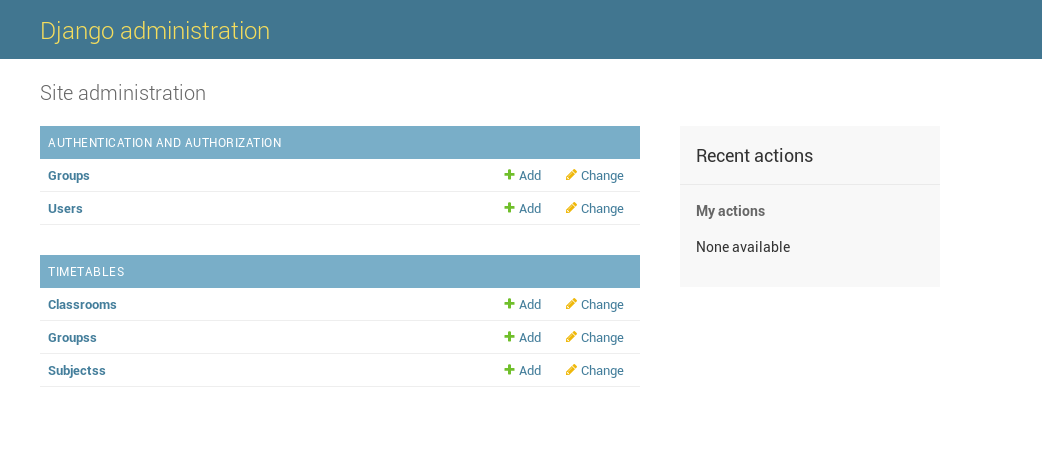
\includegraphics[width=\textwidth]{img/djangoadminpanel}
\caption{Pantalla inicial del panel de administración}
\label{djangoadminpanel}
\end{figure}

\end{enumerate} 

Por ejemplo, si a la asignatura \textit{Nuevos Paradigmas de Interacción} del \textit{Grado en Ingeniería Informática} se le añadiese una hora más de prácticas, se podría modificar tal y como se ve en la \hyperref[djangoadminmodify]{Figura \ref*{djangoadminmodify}}.

\begin{figure}
\centering
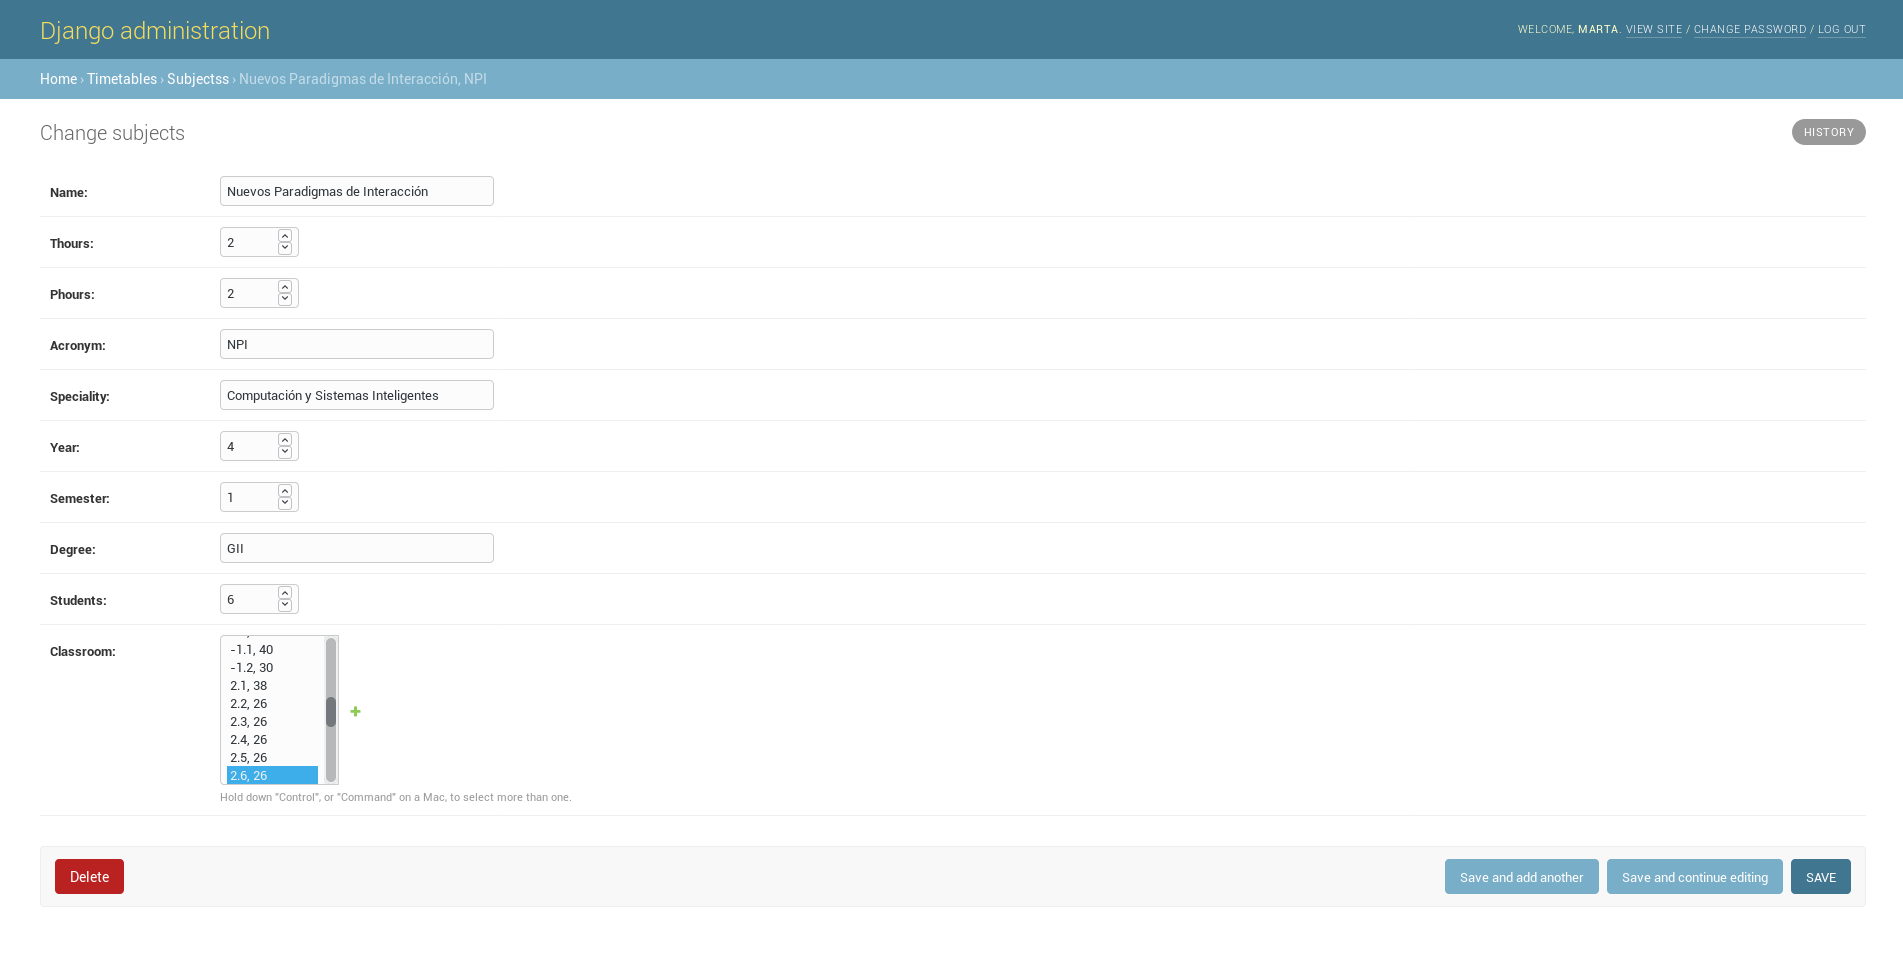
\includegraphics[width=\textwidth]{img/djangoadminmodify}
\caption{Panel para modificar la información de una asignatura}
\label{djangoadminmodify}
\end{figure}
